\documentclass[12pt,a4paper]{report}
\usepackage[left=3.5cm,top=1.5cm,right=3cm,bottom=4cm]{geometry}
\usepackage{graphicx}
\usepackage{amsmath}
\usepackage{fancyhdr}
\usepackage{cite}
\usepackage{framed}
\usepackage{a4wide}
\usepackage{float}
\usepackage{epsfig}
\usepackage{longtable}
\usepackage{enumerate}
\usepackage{afterpage}
\usepackage{multirow}
\usepackage{ragged2e}
\usepackage{gensymb}
\usepackage{amsfonts} 
\usepackage{setspace}           
\usepackage{float}
\usepackage{txfonts}
\usepackage{lipsum}
\usepackage{blindtext}
\usepackage{xpatch}
\usepackage{url}
\usepackage{leqno}
\usepackage{subcaption}
\usepackage{amsmath}
\usepackage{amssymb}
\usepackage{enumerate}
\usepackage{lscape}
\usepackage{hyperref}
\usepackage{url}
\usepackage{array} % Required for boldface (\bf and \bfseries) tabular columns
\usepackage[utf8]{inputenc}
\usepackage{multicol}
\usepackage{caption}
\usepackage{algorithm,algpseudocode}

%%%%%%%%%%%%%%%%%%%%%%%%%%%%%%%%%%%%%%%%%%%%%%%%%%%%%%%%%%%%%%%%%%%%%%%%%%%%%
%% CREATE NEW ENVT FOR MULTI-PAGE ALGORITHM %%%%%%%%%%%%%%%%%%%%%%%%%%%%%%%%%
%%%%%%%%%%%%%%%%%%%%%%%%%%%%%%%%%%%%%%%%%%%%%%%%%%%%%%%%%%%%%%%%%%%%%%%%%%%%%
\makeatletter
\newenvironment{breakablealgorithm}
{% \begin{breakablealgorithm}
	\begin{spacing}{1}
		\refstepcounter{algorithm}% New algorithm
		\hrule height.8pt depth0pt \kern2pt% \@fs@pre for \@fs@ruled
		\renewcommand{\caption}[2][\relax]{% Make a new \caption
			{\raggedright\textbf{\fname@algorithm~\thealgorithm} ##2\par}%
			\ifx\relax##1\relax % #1 is \relax
			\addcontentsline{loa}{algorithm}{\protect\numberline{\thealgorithm}##2}%
			\else % #1 is not \relax
			\addcontentsline{loa}{algorithm}{\protect\numberline{\thealgorithm}##1}%
			\fi
			\kern2pt\hrule\kern2pt
		}
	}{% \end{breakablealgorithm}
		\kern2pt\hrule\relax% \@fs@post for \@fs@ruled
	\end{spacing}
	~~ \newline
}
\makeatother
%%%%%%%%%%%%%%%%%%%%%%%%%%%%%%%%%%%%%%%%%%%%%%%%%%%%%%%%%%%%%%%%%%%%%%%%%%%%%

\newcommand{\Usefont}[1]{\fontfamily{#1}\selectfont}
\usepackage{lscape} % for landscape tables

\usepackage{hyperref}
\hypersetup{
	colorlinks=false,
	linkcolor=red,
	citecolor=red,
	pdfborder={0 0 0},
}
\usepackage{url}

\renewcommand{\baselinestretch}{1.7} 
\linespread{1.5}

\usepackage[intoc, english]{nomencl}
\hyphenpenalty=5000
\tolerance=1000

\usepackage[nottoc]{tocbibind}
\bibliographystyle{IEEEtran}
\renewcommand{\bibname}{References}

\graphicspath{{./Images/}}

%%%%%%%%%%%%%%%%%%%%%%%%%%%%%%%%%%%%%%%%%%%%%%%%%%%%%%%%%%%
%% Meta Data
%%%%%%%%%%%%%%%%%%%%%%%%%%%%%%%%%%%%%%%%%%%%%%%%%%%%%%%%%%%
\def \title{Dragon-Fly: Vehicle Surveillance System} % Project title

\def \dept{Computer Science and Engineering} %Department
\def \Degree{Bachelor of Technology} %degree
\def \branch{Computer Science and Engineering} %branch
\def \college{Government College of Engineering Kannur} % Name of the College
\def \collegeplace{Kannur} % Location of the College

\def \hod{Dr. Rafeeque P.C} %Head of Department
\def \hoddes{Professor and Head} %HOD designation

\def \acadyear{2021 - 22} % Academic year
\def \month{June 2022} %Month of Report submission
\def \date{28-06-2022} %Date of signing the declaration


\def \studentA{Abhinand C} %Project batch member 1
\def \studentAroll{KNR18CS005} % Project batch member 1 ktu id

\def \studentB{Edwin Jose George} %Project batch member 2
\def \studentBroll{KNR18CS027} % Project batch member 2 ktu id

\def \studentC{Lavanya E.V} %Project batch member 3
\def \studentCroll{KNR18CS032} % Project batch member 3 ktu id

\def \studentD{Shilpa Suresh} %Project batch member 4
\def \studentDroll{KNR18CS050} % Project batch member 4 ktu id

\def \guide{Dr. Rafeeque P.C} %Project guide
\def \guidedes{Professor}%project guide designation

\def \guideco{Prof. Bincy Antony M} %Project coguide
\def \guidecodes{Assistant Professor}%project coguide designation

\def \guideext{Prof. Project ext guide} %Project external organisation guide
\def \guideextdes{Engineer/Scientist}%project external guide designation
\def \guideextorg{External guide organization} % Project external guide organization

\def \projcordinatorA{Prof. Bincy Antony M}% Project coordinator 1 
\def \projcordinatorAdes{Assistant Professor}% Project coordinator 1 designation

\def \projcordinatorB{Prof. Bincy Antony M} % Project coordinator 2 
\def \projcordinatorBdes{Assistant Professor}% Seminar coordinator 2 designation

%%%%%%%%%%%%%%%%%%%%%%%%%%%%%%%%%%%%%%%%%%%%%%%%%%%%%%%%%%%


\begin{document}

%%%%%%%%%%%%%%%%%%%%%%%%%%%%%%%%%%%%%%%%%%%%%%%%%%%%%%%%%%%
%% FrontMatter
%%%%%%%%%%%%%%%%%%%%%%%%%%%%%%%%%%%%%%%%%%%%%%%%%%%%%%%%%%%
%==================================coverpage.tex================================
\newenvironment{coverpage}
\thispagestyle{empty}
\begin{titlepage}
	\begin{center}
		{\Usefont{phv} \Large \bf \title \par}
		\vspace*{40pt}
		\large \em \Usefont{pzc}{ 
			A Project Report \par
			Submitted to the APJ Abdul Kalam Technological University\\
			in partial fulfillment of requirements for the award of degree}\\ [0.15\baselineskip] \par 
		{\Usefont{ppl} {\bfseries \Degree}}\\
		in\\
		{\Usefont{ppl} {\bfseries \branch}}\\
		by\\
		\begin{tabular}{l c}
			\bf \studentA & \bf (\studentAroll) \\
			\bf \studentB & \bf (\studentBroll) \\
			\bf \studentC & \bf (\studentCroll) \\
			\bf \studentD & \bf (\studentDroll) \\
		\end{tabular}
		
		\vfill
		\centering
		\begin{figure}[h!]
			\centerline{
\includegraphics[scale=0.3]{gcek}}
		\end{figure}
		
		\vspace{\stretch{0.5}}
		\footnotesize{\bf DEPARTMENT OF COMPUTER SCIENCE AND  ENGINEERING} \par
		\bf{GOVERNMENT COLLEGE OF ENGINEERING KANNUR} \par
		\bf{KERALA} \par
		\bf{\month}
	\end{center}		
\end{titlepage}	


% To print name of only the project coordinator 1 in the certificate page
%==================================certificate1.tex================================
% To print name of only the seminar coordinator 1 in the certificate page

\newenvironment{certificate}

	\newpage
	\begin{center}	
		%\vspace{1.5cm}
		
	\textbf{DEPARTMENT OF COMPUTER SCIENCE AND ENGINEERING}
	\textbf{GOVERNMENT COLLEGE OF ENGINEERING } 
	\textbf{KANNUR}
		
		\textbf{\acadyear} 
	\end{center}
	
	\begin{center}
		
\includegraphics[scale=0.3]{gcek}	
	\end{center}
	\begin{center}
		\textbf{CERTIFICATE}
	\end{center}
	
	This is to certify that the report entitled \textbf{\title} submitted by \textbf{\studentA} \space (\studentAroll), \textbf{\studentB} \space (\studentBroll), \textbf{\studentC} \space (\studentCroll) \& \textbf{\studentD} \space (\studentDroll) to the APJ Abdul Kalam Technological University in partial fulfillment of the B.Tech.\ degree in \branch \hspace*{2pt} is a bonafide record of the project work carried out by him under our guidance and supervision. This report in any form has not been submitted to any other University or Institute for any purpose.
	
	\vfill
	\begin{singlespace}
		\begin{tabular}{p{0.29\textwidth} p{0.29\textwidth} p{0.29\textwidth}}
			
			\begin{tabular}[c]{@{}c@{}}
				\textbf{\guide}\\
				(Project Guide)\\
				\guidedes \\
				Dept.of CSE\\
				Govt. College of Engineering\\
				Kannur
			\end{tabular}
		
			&&
			\begin{tabular}[c]{@{}c@{}}
				\textbf{\hod}\\
				(Head of Dept.) \\
				Professor\\
				Dept.of CSE\\
				Govt. College of Engineering\\
				Kannur
			\end{tabular} \\
		
			& 
			\begin{tabular}[c]{@{}c@{}}
				\textbf{\projcordinatorA}\\
				(Project Coordinator)\\
				\projcordinatorAdes \\
				Dept.of CSE\\
				Govt. College of Engineering\\
				Kannur
			\end{tabular}
			&
	\end{tabular}

	\end{singlespace}
	
	\thispagestyle{empty}



 

% To print names of both the project coordinators in the certificate page
%\include{SupportMatter/certificate2}

%==================================declaration.tex================================
%
\newpage
\newenvironment{declaration}
\thispagestyle{empty}
\begin{center}
\vspace*{50pt}
\textbf{DECLARATION}\\
\end{center}
We hereby declare that the project report {\bf{\title}}, submitted for partial fulfillment of the requirements for the award of degree of Bachelor of Technology of the APJ Abdul Kalam Technological University, Kerala is a bonafide work done by us under supervision of \guide \hspace*{2pt} \par
This submission represents our ideas in our own words and where ideas or words of others have been included, we have adequately and accurately cited and referenced the original sources.\par 
We also declare that we have adhered to ethics of academic honesty and integrity and have not misrepresented or fabricated any data or idea or fact or source in my submission. We understand that any violation of the above will be a cause for disciplinary action by the institute and/or the University and can also evoke penal action from the sources which have thus not been properly cited or from whom proper permission has not been obtained. This report has not been previously formed the basis for the award of any degree, diploma or similar title of any other University.

\noindent \begin{minipage}{0.45\linewidth}
\begin{flushleft}
\vspace{2.5cm}

\collegeplace \\
\date

\end{flushleft} 
\end{minipage}
\hfill
\begin{minipage}{0.45\linewidth}
\begin{flushright}                                      
\vspace{1.5cm}

\textbf{\studentA}\\
\textbf{\studentB}\\
\textbf{\studentC}\\
\textbf{\studentD}\\


\end{flushright} 
\end{minipage}
\thispagestyle{empty}


\pagenumbering{roman} 

%============================= abstract.tex================================
\chapter*{Abstract}%
%\addcontentsline{toc}{chapter}{\numberline{}Abstract}%
\addcontentsline{toc}{chapter}{Abstract}%

Vehicles are one of the most important means of transport. It have seen large improvements and innovation in the past decades. Almost all of our day-to-day activities are depended on the transport system. Hence there exist the need for safe policing of traffic. Existing method involves large human resource allocated for tedious task of tracking a vehicle. This project proposes an integrated system that make use of existing state-of-the-art technologies to support policing of traffic. The system incorporates the use of AI technologies to mimic the human intelligence for faster processing of tedious task. Major AI technologies mention in this project include YOLOv4 algorithm, DeepSORT tracker and Siamese Network. The system aims for successful re-identification of multiple vehicles across multiple camera viewpoints. The system provides interactive user interface that hides the complexities involved in achieving the task. Various aspects of security are also considered during the development of the project.
\vfill
\begin{flushright}
	\textit{\studentA} \\
	\textit{\studentB} \\
	\textit{\studentC} \\
	\textit{\studentD}
\end{flushright}

\thispagestyle{plain}
%=======================================================================

\chapter*{Acknowledgments}
 \lipsum[1-2]
 

\hfill Project Team 

\thispagestyle{empty}
\newpage

%%**********************Table of Contents***********************
\tableofcontents
\listoffigures
\listoftables

%%%%%%%%%%%%%%%%%%%%%%%%%%%%%%%%%%%%%%%%%%%%%%%%%%%%%%%%%%%
%% Main Content
%%%%%%%%%%%%%%%%%%%%%%%%%%%%%%%%%%%%%%%%%%%%%%%%%%%%%%%%%%%
\cleardoublepage
\setcounter{page}{1}
\pagenumbering{arabic}

\clearpage
\chapter{Introduction}

Vehicles are one of the most important means of road transport for goods and services. Almost all the countries around the world have complicated road networks connecting remote locations. These road networks facilitate easy transport of people, goods, and services further encouraging the development of more networks. There has been exponential growth in the automobile industry to provide and market various automobiles into these road networks. This requires the need of policing this sector to ensure the safety of the people and the country. Controlling and managing this huge network is a great challenge due to its very vast and complicated network supporting a large population of vehicles. As part of policing, cameras are set up at various locations to monitor the traffic. However there exist the tedious work of manually analyzing the camera feed to detect and control the traffic. This project aims to tackle this particular issue.

\section{Problem Statement}
A novel approach to provide an integrated platform utilizing existing infrastructure to monitor transport sector, and extend timely information to policing agencies, with intuitive interface.

\section{Background}
Road traffic is one of the dynamic public sectors that involve huge human interventions. These include, but are not limited to construction of roads, transport of goods and other products, general public using public and private travel means, movement of construction goods, etc. The automobile is a booming industry, with a lot of companies producing new automobiles for the market meeting the need of the public. These include construction vehicles such as JCB, tractors, excavators, road rollers, trucks, etc; public goods vehicles such as vans, trucks, pickups; public vehicles such as buses, autos, taxis, etc; private vehicles such as cars, bikes, etc. Manufactures continuously supply new and modern automobiles to support the day-to-day activities of the public, and hence the nation.

This huge flow of vehicles demanded the setting up of rules and regulations for the safety of the people and properties. These rules ensured a smooth flow of traffic. However, at times these rules are broken by the public. To re-enforce these regulations proper policing is required. Officials are deployed at various points to physically inspect and regulate traffic. Upon finding any violation, the offender is fined. With the involvement of technology, speed cameras are set up on major roads to ensure that all vehicles do not travel beyond the safe speed limit. These cameras are special cameras that are triggered only upon finding a vehicle moving at high speed. When triggered they capture the license plate of the vehicle along with the time and place of the event. Obtaining license plate info helps to fetch associated vehicle information such as owner, address, vehicle make, model, type, etc. However, these are special cameras and a too costly to be deployed in larger and remote places.

At times, it was necessary to re-trace the route followed by a particular vehicle. As the technology grew, surveillance cameras are set up at various locations. Cameras allowed continuous monitoring of a particular section of the road. The feeds are saved at the severs and officials can replay the tape to extract the necessary information. These cameras are far less expensive than the speed cam, but also have lower resolution. These cameras find it difficult to extract unique features such as license plate information. They are mainly used for surveillance purposes with the just aim to record the event occurring in a fixed sector.  

As the camera network was set up, the process of policing is still a tedious task. Officials need to manually replay each camera feed. Most of the time, the feed would be empty showing there was no traffic at that moment. Moreover, there would be many types of vehicles to consider. It is also possible for the vehicles to take alternative routes. The manual process of monitoring each feed is a highly time-consuming and tired-sum process. Moreover, it may need to identify a particular vehicle before it travels out of a particular zone.

This calls for the need for a system that could traverse the camera network detecting useful video frames and analyzing them to extract relevant information. This information can include features like type, color, model, location, time of the event, etc. A query can be issued to look up vehicles matching such descriptions. This saves a lot of time by skipping the dead frames. Another advantage is that, during an investigation, the witness can only provide such features to testimony an event. The suspect may be able to forge the license plate, but not the whole vehicle description. 



\section{NVIDIA AI City Challenge}
This project is one of the open challenges in NVIDIA AI city challenge, to perform Natural language-based vehicle track retrieval and City-scale multi-camera vehicle tracking. Various research and study are being conducted on this field.

\subsection*{Definition}
AI City means applying AI to improve the efficiency of operations in city environments. This manifests itself in improving transportation outcomes by making traffic more efficient and making roads safer, improving building operations by making them more energy efficient, reducing friction in retail environments by speeding up traffic at retail checkout, etc. The common thread in all these diverse uses of AI is the extraction of actionable insights from a plethora of sensors through real-time streaming and batch analytics of the vast volume and flow of sensor data, such as those from cameras.

\subsection*{The AI City Challenge Workshop 2022}
The AI City Challenge Workshop at CVPR 2022 specifically focus on problems in two domains where there is tremendous unlocked potential at the intersection of computer vision and artificial intelligence
\begin{enumerate}
	\item The Intelligent Traffic Systems (ITS)
	\begin{itemize}
		\item City-scale multi-camera vehicle tracking
		\item Natural language-based vehicle track retrieval
		\item Naturalistic driver data analytics
		\item Anomaly Detection
	\end{itemize}
	\item The Brick and Motar retail business
	\begin{itemize}
		\item Automated checkout
		\item Efficient Store utilization
	\end{itemize}
\end{enumerate}

\section{Application}
Mere processing of footage from camera have wide range of applications, especially in an dynamic sector like road transport. Due to urbanization and expansion of road networks, supported by the growth of technology and digitization, applications can vary from monitoring, planning to research, security and decision making. Some of the possible application of analyzing the traffic using camera network are:
\begin{itemize}
	\item Identify and track the route taken by a targeted vehicle.
	\item Identify violations such as the check for helmet and passenger count in two wheeler, illegal turn taken at one-way roads, non-permitted vehicle entering the perimeter (eg: heavy trucks via old bridge is prohibited) etc.
	\item Identify events such as accidents or unexpected crowding, etc.
	\item Conduct research on the flow of traffic aiding for decision making for new road construction.
	\item Provide decision parameter for efficient routing of traffic to remove traffic blocks. Helps to change traffic load for emergency services such as ambulance, fire-trucks etc.
	\item Can be used to checkpoint vehicles, enhancing integrity and security of services. For example:
	\begin{itemize}
		\item Confirming that cargo have left the station and is in-route to its destination.
		\item Track and predict public transport services.
	\end{itemize}
\end{itemize}
\chapter{Literature Review} 
Artificial Intelligence (AI) is one of the most researched topic in the domain of Computer Science. It is the artificial creation of human-like intelligence that can learn, perceive and process information. AI provides a powerful tool for solving image recognition, document classification as well as for the advancement of interdisciplinary problems. AI is an interdisciplinary domain that make use of various mathematical models, statistical models, neural networks etc to learn pattern and predict unseen data with comparable accuracy. Unlike traditional model, they learn the concepts and rules by learning from examples. Traditional model requires rules to be specified, that results in higher computation but higher accuracy. The ability of AI to generalize even accounting for noise with higher speed promoted various levels of growth, especially in the field of image processing.

Image processing is an interesting field of study that involves image classification, object detection, instance segmentation, object tracking etc. There have been various research and study to overcome the traditional image processing that employ various algorithm using opencv. Various level of optimization was performed to build deep neural networks that can effectively extract relevant features to identify the object.

\section{Vehicle Identification Systems}
AI have always found it way in developing intelligent system in automobile industry. They are used for smarter manufacturing process, leading to design of efficient systems. They have also helped in business by recommending most efficient path in road network. They are also utilized to build intelligent autonomous vehicles that can react to changes in real-time environment and make way to its destination safely. AI is also used for monitoring purposes for enhancing security. Several parallel papers and researches are build developing such monitoring system using camera network. Below presented are few of such system that are deployed in selected area.

\subsection{CityFlow}
Urban traffic optimization using traffic cameras as sensors is driving the need to advance state-of-the-art multitarget multi-camera (MTMC) tracking. This work  introduces CityFlow \cite{Tang_2019_CVPR}, a city-scale traffic camera dataset having the largest-scale dataset in terms of spatial coverage and the number of cameras/videos in an urban environment. The dataset contains a wide range of scenes, viewing angles, vehicle models, and urban traffic flow conditions. Camera geometry and calibration information are provided to aid spatio-temporal analysis. In addition, a subset of the benchmark is made available for the task of image-based vehicle re-identification (ReID). It also opens a way for new research problems such as vehicle pose estimation, viewpoint generation, etc.

It have compared and bench-marked several state-of-the-art models using Muiti-Target-Single-Camera and Multi-Target-Multi-Camera tracking. They have given emphasis on the visual-spacio-temporal reasoning to re-identification. This approach was able to product better and faster results, handle large scale recognition and is successful in conducting small predictions. However, they require multiple camera scanning same object at multi viewpoint at the same time. It also demanded high quality videos and was also set-up at junction points.

\subsection{Vehicle Make and Model Recognition system}
A Vehicle Make and Model Recognition (VMMR) system \cite{manzoor2019real} can provide great value in terms of
vehicle monitoring and identification based on vehicle appearance in addition to the vehicles attached license plate typical recognition. A VMMR system has a unique set of challenges and issues. Few of the challenges are image acquisition, variations in illuminations and weather, occlusions, shadows, reflections, large variety of vehicles, inter-class and intra-class similarities, addition/deletion of vehicles models over time, etc. The system extract image features from vehicle images and create feature vectors to represent the dataset. Then, two classification algorithms, Random Forest (RF) and Support Vector Machine (SVM) are used for classification. The proposed VMMR system recognizes vehicles on the basis of make, model, and generation (manufacturing years).

For feature extraction, HOG and GIST algorithm are utilized. These vectors are saved in database supporting faster processing speed and improved recognition accuracy, accounting for partial viewpoints. However they have limited region interest with high computation time with increase in block of HOG. The system only addresses local high dimensional features, and have no global representation.

\subsection{Multi-level Feature extraction}
The intelligent transportation system is currently an active research area, and vehicle
re-identification (Re-Id) is a fundamental task to implement it. It determines whether the given vehicle image obtained from one camera has already appeared over a camera network or not. This task becomes more challenging because of intra-class similarity,
viewpoint changes, and inconsistent environmental conditions. A system \cite{cai2019efficient} is proposed which re-identifies a vehicle in two steps: first, shortlist the vehicle from a gallery set on the basis of appearance, and then in the second step, verify the shortlisted vehicle’s license plates with a query image to identify the targeted vehicle. 

The global channel extracts the feature vector from the whole vehicle image, and the local region channel extracts more discriminative and salient features from different regions. A Siamese neural network is used to verify license plates to reach the
exact vehicle. The system also account for color, model, and type as parameters of feature vectors. However, a significant impact of illumination can be found, which is worsen by background clutter. It also do not account for cross camera vehicle tracking.

\subsection{Trends in Vehicle Re-Identification}
Vehicle Re-identification (re-id) over surveillance camera network with non-overlapping
field of view is an exciting and challenging task in intelligent transportation systems (ITS). Vehicle re-id matches targeted vehicle over non-overlapping views in multiple camera network. However, it becomes more difficult due to inter-class similarity, intra-class variability, viewpoint changes, and spatio-temporal uncertainty. In order to draw a detailed picture of vehicle re-id research, this research \cite{deng2021trends} provides a comprehensive description of the various vehicle re-id technologies, applicability, datasets, and a brief comparison of different methodologies. 
This research specifically focuses on vision-based vehicle re-id approaches, including vehicle appearance, license plate, and spatio-temporal characteristics. Some of the main technology taken under consideration are:
\begin{enumerate}
	\item Magnetic Sensor-Based Vehicle Re-Identification
	\item Inductive Loop-Based Vehicle Re-Identification
	\item Global Positioning Systems-Based Vehicle Re-Identification
	\item Vision-Based Vehicle Re-Identification
	\begin{enumerate}
		\item Feature Representation for Vehicle Re-Identification
		\item Traditional Machine Learning-Based Vehicle Re-Identification
		\item Similarity Metric for Vehicle Re-Identification
		\item Fine-Grained Visual Recognition-Based Vehicle Re-Identification
		\item View-Aware-Based Vehicle Re-Identification
		\item Generative Adversarial Network-Based Vehicle Re-Identification
		\item Attention Mechanism
		\item License Plate-Based Vehicle Re-Identification
	\end{enumerate}
	\item Spatio-Temporal Cues-Based Vehicle Re-Identification Approaches
	\item Hybrid Methods-Based Vehicle Re-Identification
\end{enumerate}


\section{Traditional Methods of Image processing}
Traditional methods are computation intensive and hence slow. However, they have higher accuracy, but prone to noise. Some of the methods are:
\begin{enumerate}
	\item Harris Algorithm \\
			Corner detection algorithm that identifies and compares the corners of objects and then compute the similarity.
	\item SIFT: Scale Invariant Feature Transform\\
			Key-points of objects are first extracted from a set of reference images[1] and stored in a database. An object is recognized in a new image by individually comparing each feature from the new image to this database and finding candidate matching features based on Euclidean distance of their feature vectors. 
	\item HOG: Histogram of Oriented Gradients \\
			It counts occurrences of gradient orientation in localized portions of an image, computed on a dense grid of uniformly spaced cells and uses overlapping local contrast normalization for improved accuracy.
	\item GLOH: Gradient Location and Orientation Histogram \\
			It is a SIFT-like descriptor that considers more spatial regions for the histograms. An intermediate vector is computed from Location and orientation bins, for different dimensions.
	\item Canny Edge detection \\
		It is a technique to extract useful structural information from different vision objects and dramatically reduce the amount of data to be processed.
	\item SURF: Speed-ed Up Robust Features \\
			It is a fast and robust algorithm for local, similarity invariant representation and comparison of images. The main interest of the SURF approach lies in its fast computation of operators using box filters, thus enabling real-time applications such as tracking and object recognition. 
	\item DPM: Deformable Parts Model \\
			Special case of Dalal and Triggs Detector, making improvement over HOG and Support Vector Machine (SVM). Figure \ref{fig:dpm} shows the steps for detection of human.
\end{enumerate} 


\begin{figure}[!ht]
	\centering
	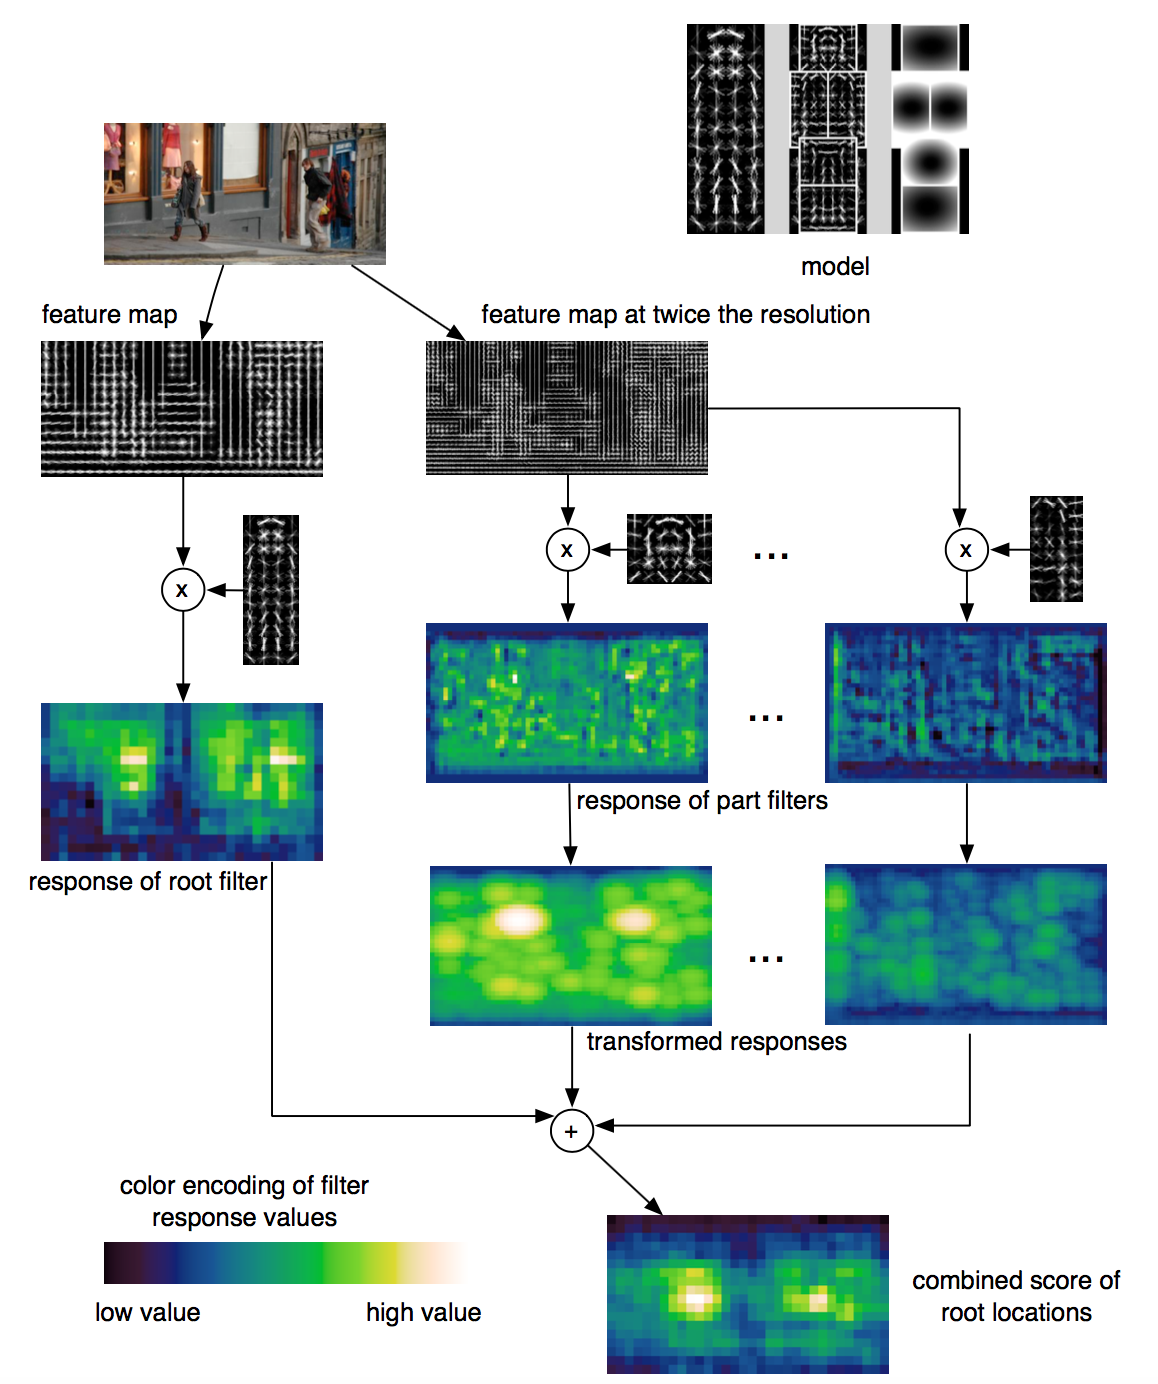
\includegraphics[width=0.7\linewidth]{Images/DPM}
	\caption{Deformable Parts Model for Human detection}
	\label{fig:dpm}
	%SRC: https://github.com/lilianweng/lilianweng.github.io/blob/master/posts/2017-12-15-object-recognition-part-2/DPM-matching.png

\end{figure}

\section{Neural Network Models}
Neural Network model consists of neurons firing signals to change the output. Each neuron have weights associated along with activation function. The learning happens through the change of each weights. They require higher training time, but produce output faster along with the ability to resist the effect of noise. They generalize well event to identify occluded objects from image. 

The major jump from traditional method into network model was on to the introduction of AlexNet Model. AlexNet have 5 convolution layers that effectively scale and extract the features. They are then pooled at each layers. At the end, a dense neural network gets trained to predict values for the output neuron, which are softmax-ed to obtain particular class. Dense neural network mimics a classifier. They are used for image classification. To account for various dimension of image, a concept of image pyramid is used to process image at various levels. VGG is an extension of AlexNet. Figure \ref{fig:alexnet_vgg} shows the architecture of AlexNet and VGG model. Convolutional Neural Network (CNN) is a set of filters that extract a specific feature by applying some kernel.<

\begin{figure}[!ht]
	\centering
	\begin{tabular}[!ht]{m{0.4\hsize}m{0.55\hsize}}
		\begin{subfigure}[b]{\linewidth}
			\centering
			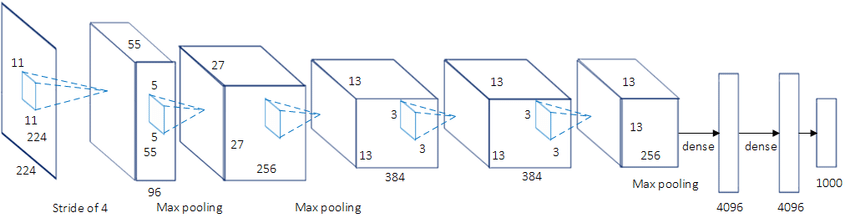
\includegraphics[width=0.9\linewidth]{Images/AlexNet_3D}
			\caption{AlexNet Architecture}
			% SRC: https://www.researchgate.net/figure/AlexNet-Convolutional-Neural-Network-architecture-Figure-reproduced-from-14_fig1_316450908
		\end{subfigure}
		
		\begin{subfigure}[b]{\linewidth}
			\centering
			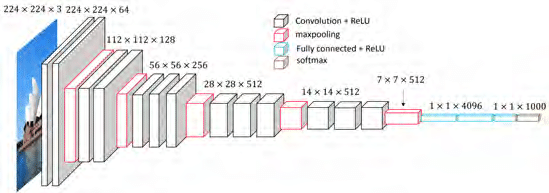
\includegraphics[width=0.9\linewidth]{Images/VGG_3D}
			\caption{VGG Architecture}
			% SRC: https://www.researchgate.net/figure/The-architecture-of-a-VGGNet-CNN-after-Wang-et-al-2017_fig1_323796590
		\end{subfigure}
	
		& 
		\begin{subfigure}[b]{\linewidth}
			\centering
			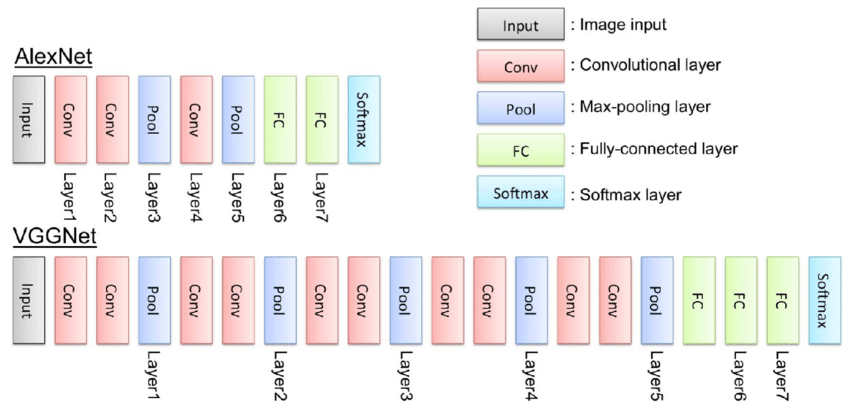
\includegraphics[width=\linewidth]{Images/AlexNet-and-VGGNet-architecture}
			\caption{Layers of model. Classification done by FC layers}
			%SRC: https://www.researchgate.net/figure/AlexNet-and-VGGNet-architecture_fig1_282270749
		\end{subfigure}
	\end{tabular}
	\caption{AlexNet \& VGG Model}	
	\label{fig:alexnet_vgg}
\end{figure}

Owing to the success of AlexNet and VGG model, various study and research are conducted on the CNN layers to efficiently extract features. Some of the major contributions are summarized below.

\subsubsection{Overfeat}
\begin{itemize}
	\item Problem addressed
		\begin{itemize}
			\item CNN network can accept only fixed size images. To process a large image, the image needs to be cropped and resized to fit the dimension of the input of the network. The size constraint is imposed not because of the input layers, but due to the FC layers.
			\item One solution involves manually cropping the image and feeding the network, a stimulation of sliding window. It involves redundant calculation at the image pixels.
		\end{itemize}
	\item Solution Proposed
		\begin{itemize}
			\item Implementation of FC as Conv network, removing the input constraint
			\item Image pyramid of 6 sizes [ 461*569 , 425*497 , 386*461 , 317*389 , 281*317 , 245*245 ] creating spatial output dimensions. The spacial output dimensions show how many object can be detected from the image
		\end{itemize}
\end{itemize}

\begin{figure}[h!]
	\centering
	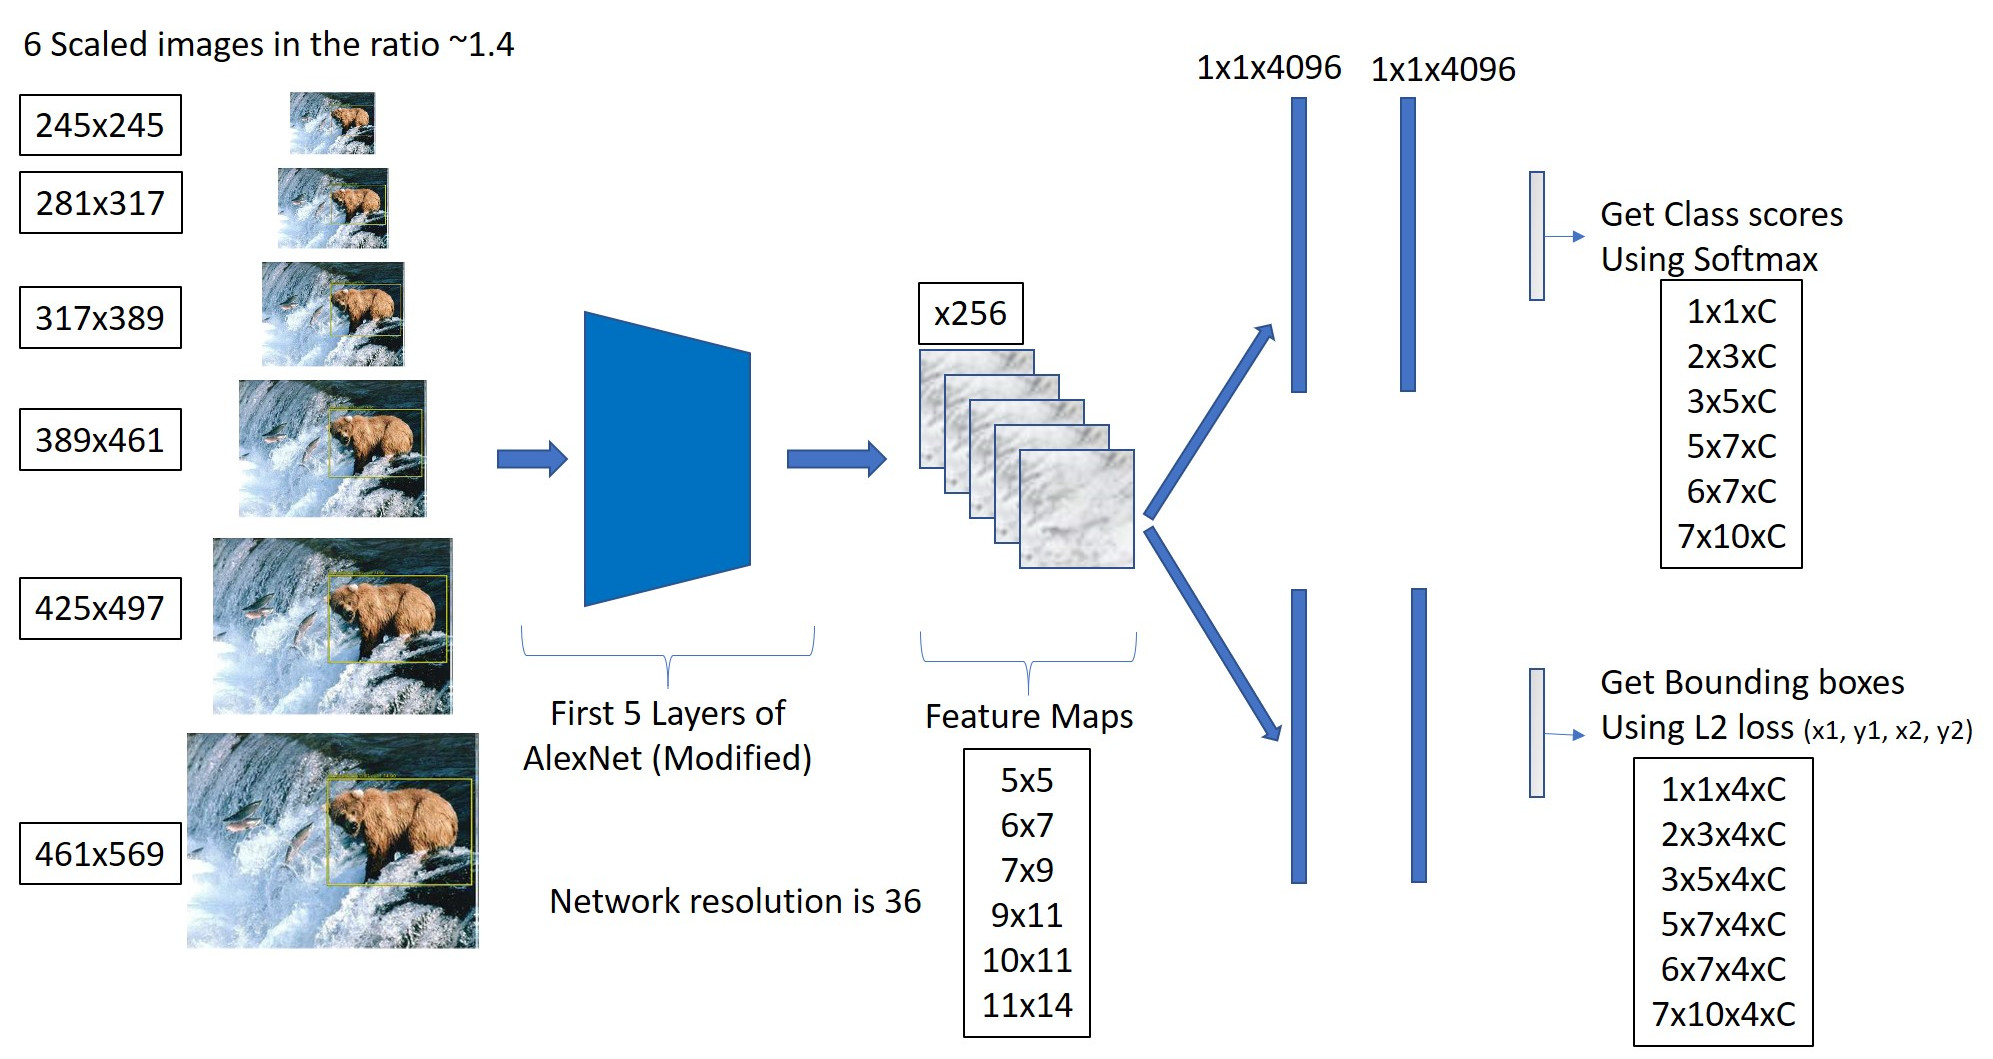
\includegraphics[width=0.9\linewidth]{Images/overfeat}
	\caption{Overfeat Architecture}
	%SRC: https://cogneethi.com/assets/images/evodn/detection_overfeata_detect.jpg
\end{figure}

\subsubsection{R-CNN: Regions with Convolutional Neural Networks}
%SRC: https://towardsdatascience.com/r-cnn-fast-r-cnn-faster-r-cnn-yolo-object-detection-algorithms-36d53571365e
To bypass the problem of selecting a huge number of regions, we can use selective search to extract just 2000 regions from the image - called region proposals. These 2000 region proposals are generated using the selective search algorithm. These 2000 candidate region proposals are warped into a square and fed into a convolutional neural network that produces a 4096-dimensional feature vector as output. The CNN acts as a feature extractor and the output dense layer consists of the features extracted from the image and the extracted features are fed into an SVM to classify the presence of the object within that candidate region proposal. The algorithm also predicts four values which are offset values to increase the precision of the bounding box. Some of the drawbacks are
\begin{itemize}
	\item It still takes a huge amount of time to train the network as we would have to classify 2000 region proposals per image.
	\item It cannot be implemented real time as it takes around 47 seconds for each test image.
	\item The selective search algorithm is a fixed algorithm. Therefore, no learning is happening at that stage. This could lead to the generation of bad candidate region proposals.
\end{itemize}

\begin{figure}[h!]
	\centering
	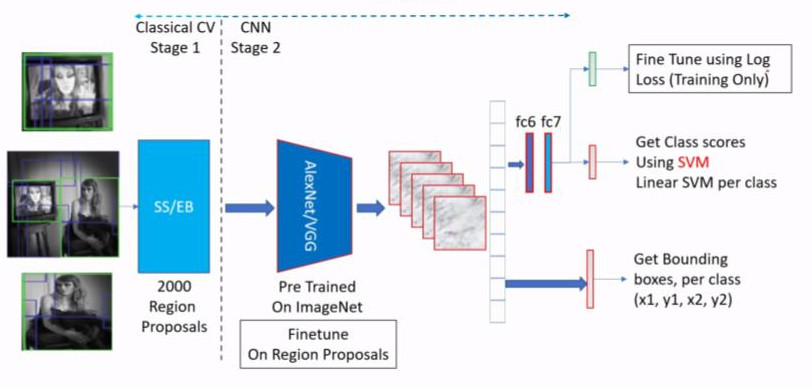
\includegraphics[width=0.9\linewidth]{Images/RCNN}
	\caption{R-CNN model}
	\label{fig:rcnn}
\end{figure}

The same author of the previous paper(R-CNN) solved some of the drawbacks of R-CNN to build a faster object detection algorithm and it was called \textbf{Fast R-CNN}. The approach is similar to the R-CNN algorithm. But, instead of feeding the region proposals to the CNN, we feed the input image to the CNN to generate a convolutional feature map. From the convolutional feature map, we identify the region of proposals and warp them into squares and by using a RoI pooling layer we reshape them into a fixed size. From the RoI feature vector, softmax layer is used to predict the class of the proposed region and also the offset values for the bounding box. “Fast R-CNN” is faster than R-CNN is because we do not need to feed 2000 region proposals to the CNN every time. Instead, the convolution operation is done only once per image and a feature map is generated from it.

Both of the above algorithms(R-CNN \& Fast R-CNN) uses selective search to find out the region proposals. Selective search is a slow and time-consuming process affecting the performance of the network. Therefore an object detection algorithm was proposed in \textbf{Faster-RCNN} that eliminates the selective search algorithm and lets the network learn the region proposals. Similar to Fast R-CNN, the image is provided as an input to a convolutional network which provides a convolutional feature map. Instead of using selective search algorithm on the feature map to identify the region proposals, a separate network is used to predict the region proposals. The predicted region proposals are then reshaped using a RoI pooling layer which is then used to classify the image within the proposed region and predict the offset values for the bounding boxes.

\subsection{YOLO: You Only Look Once}
YOLO \cite{yolo_core_paper} is a clever CNN for doing object detection in real-time. The algorithm applies a single neural network to the full image, and then divides the image into regions and predicts bounding boxes and probabilities for each region. These bounding boxes are weighted by the predicted probabilities. The algorithm “only looks once” at the image in the sense that it requires only one forward propagation pass through the neural network to make predictions. After non-max suppression it then outputs recognized objects together with the bounding boxes. With YOLO, a single CNN simultaneously predicts multiple bounding boxes and class probabilities for those boxes. YOLO trains on full images and directly optimizes detection performance. 

\subsubsection{Steps}
\begin{enumerate}
	\item YOLO is based on the idea of segmenting an image into smaller images. The image is split into a square grid of dimensions $S*S$. The cell in which the center of an object resides, is the cell responsible for detecting that object. 
	
	\item Each cell will predict $B$ bounding boxes and a confidence score for each box. Each of these bounding boxes is made up of 5 numbers: the x position, the y position, the width, the height, and the confidence. 
	
	\item The coordinates $(x, y)$ represent the location of the center of the predicted bounding box, and the width and height are fractions relative to the entire image size. The confidence represents the Intersection Over Union (IOU) between the predicted bounding box and the actual bounding box, referred to as the ground truth box. 
	
	\item Each cell also predicts the class of the object. This class prediction is represented by a one-hot vector length $C$, the number of classes in the dataset. However, while each cell may predict any number of bounding boxes and confidence scores for those boxes, it only predicts one class. 
	
	\item Each prediction from a grid cell will be of shape $C + B * 5$. Because there are $S*S$ grid cells in each image, the overall prediction of the model is a tensor of shape $S*S*(C+B*5)$.
\end{enumerate}
\begin{figure}[H]
	\centering
	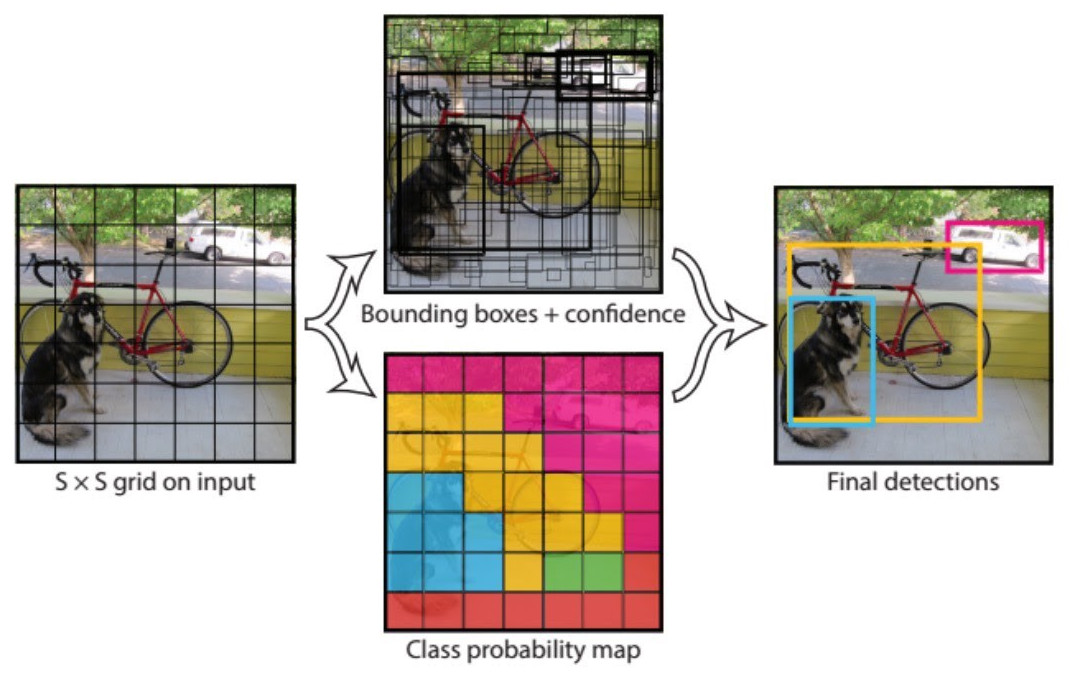
\includegraphics[width=0.7\linewidth]{Images/yolo_steps}
	\caption{YOLO detection steps}
	%SRC: https://towardsdatascience.com/evolution-of-yolo-yolo-version-1-afb8af302bd2
\end{figure}

\subsubsection{Architecture}
The YOLO model is made up of three key components:
\begin{enumerate}
	\item The Backbone \\
	It is the part of the network made up of convolutional layers to detect key features of an image and process them. The backbone is first trained on a classification dataset and typically trained at a lower resolution than the final detection model, as detection requires finer details than classification. YOLOv4 have CSP-Darknet-53 as the backbone of the network 

	\item The Neck \\
	It uses the features from the convolution layers in the backbone with fully connected layers to make predictions on probabilities and bounding box coordinates. 
	
	\item The Head \\
	It is the final output layer of the network which can be interchanged with other layers with the same input shape for transfer learning. 	
\end{enumerate} 
These three portions of the model work together to first extract key visual features from the image then classify and bound them. This happens for multiple scales. Each YOLO head corresponds to particular scale of detection. They are the combined on score values to produce final detection. Figure \ref{fig:yolov4-architecture} shows the architecture of YOLOv4 model.

\begin{figure}[H]
	\centering
	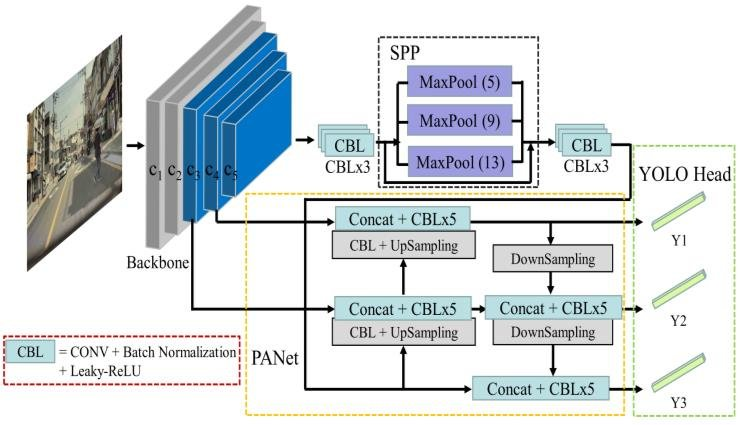
\includegraphics[width=0.85\linewidth]{Images/YOLOV4-research-gate}
	\caption{YOLOv4 architecture}
	\label{fig:yolov4-architecture}
	%SRC: https://www.researchgate.net/figure/Overall-structure-of-YOLOv4-including-CSPDarknet-backbone-SPPnet-PANet-and-3-YOLO_fig2_344919620
\end{figure}


\subsubsection{YOLO variants}
\begin{table}[H]
	\centering
	\begin{tabular}{|c|c|c|c|c|}
		\hline
		\textbf{Varient} & \textbf{Release} & \textbf{FPS} & \textbf{mAP} & \textbf{Feature Extractor} \\ \hline
		\begin{tabular}[c]{@{}c@{}}YOLOv1\\ (448*448)\end{tabular} & \begin{tabular}[c]{@{}c@{}}6 May 2016\\ Joseph Redmon\end{tabular} & 45 & 63.4 & \begin{tabular}[c]{@{}c@{}}24 CNN\\ 2 FC\end{tabular} \\ \hline
		\begin{tabular}[c]{@{}c@{}}YOLOv2\\ (416*416)\end{tabular} & \begin{tabular}[c]{@{}c@{}}25 Dec 2016\\ Joseph Redmon\end{tabular} & 67 & 76.8 & VGG-16 \\ \hline
		\begin{tabular}[c]{@{}c@{}}YOLOv3\\ (416*416)\end{tabular} & \begin{tabular}[c]{@{}c@{}}8 April 2018\\ Joseph Redmon\end{tabular} & 35 & 55.3 & Darknet-53 \\ \hline
		\begin{tabular}[c]{@{}c@{}}YOLOv4\\ (416*416)\end{tabular} & \begin{tabular}[c]{@{}c@{}}23 April 2020\\ Alexey Brochkovskiy\end{tabular} & 38 & 62.8 & CSPDarknet-53 \\ \hline
		YOLOv5 & \begin{tabular}[c]{@{}c@{}}18 May 2020\\ Glenn Jocher\end{tabular} & 70.9 & 66.9 & CSPDarknet-53 \\ \hline
		\begin{tabular}[c]{@{}c@{}}PP-YOLO\\ (416*416)\end{tabular} & \begin{tabular}[c]{@{}c@{}}3 August 2020\\ Xiang Long\end{tabular} & 72.9 & 62.8 & ResNet50-vd-dcn \\ \hline
	\end{tabular}
	\caption{YOLO variants comparison}
\end{table}

\chapter{System Development}
\lipsum[1]


\section{System Architecture}
\lipsum[1-2]

\begin{figure}
	\centering
	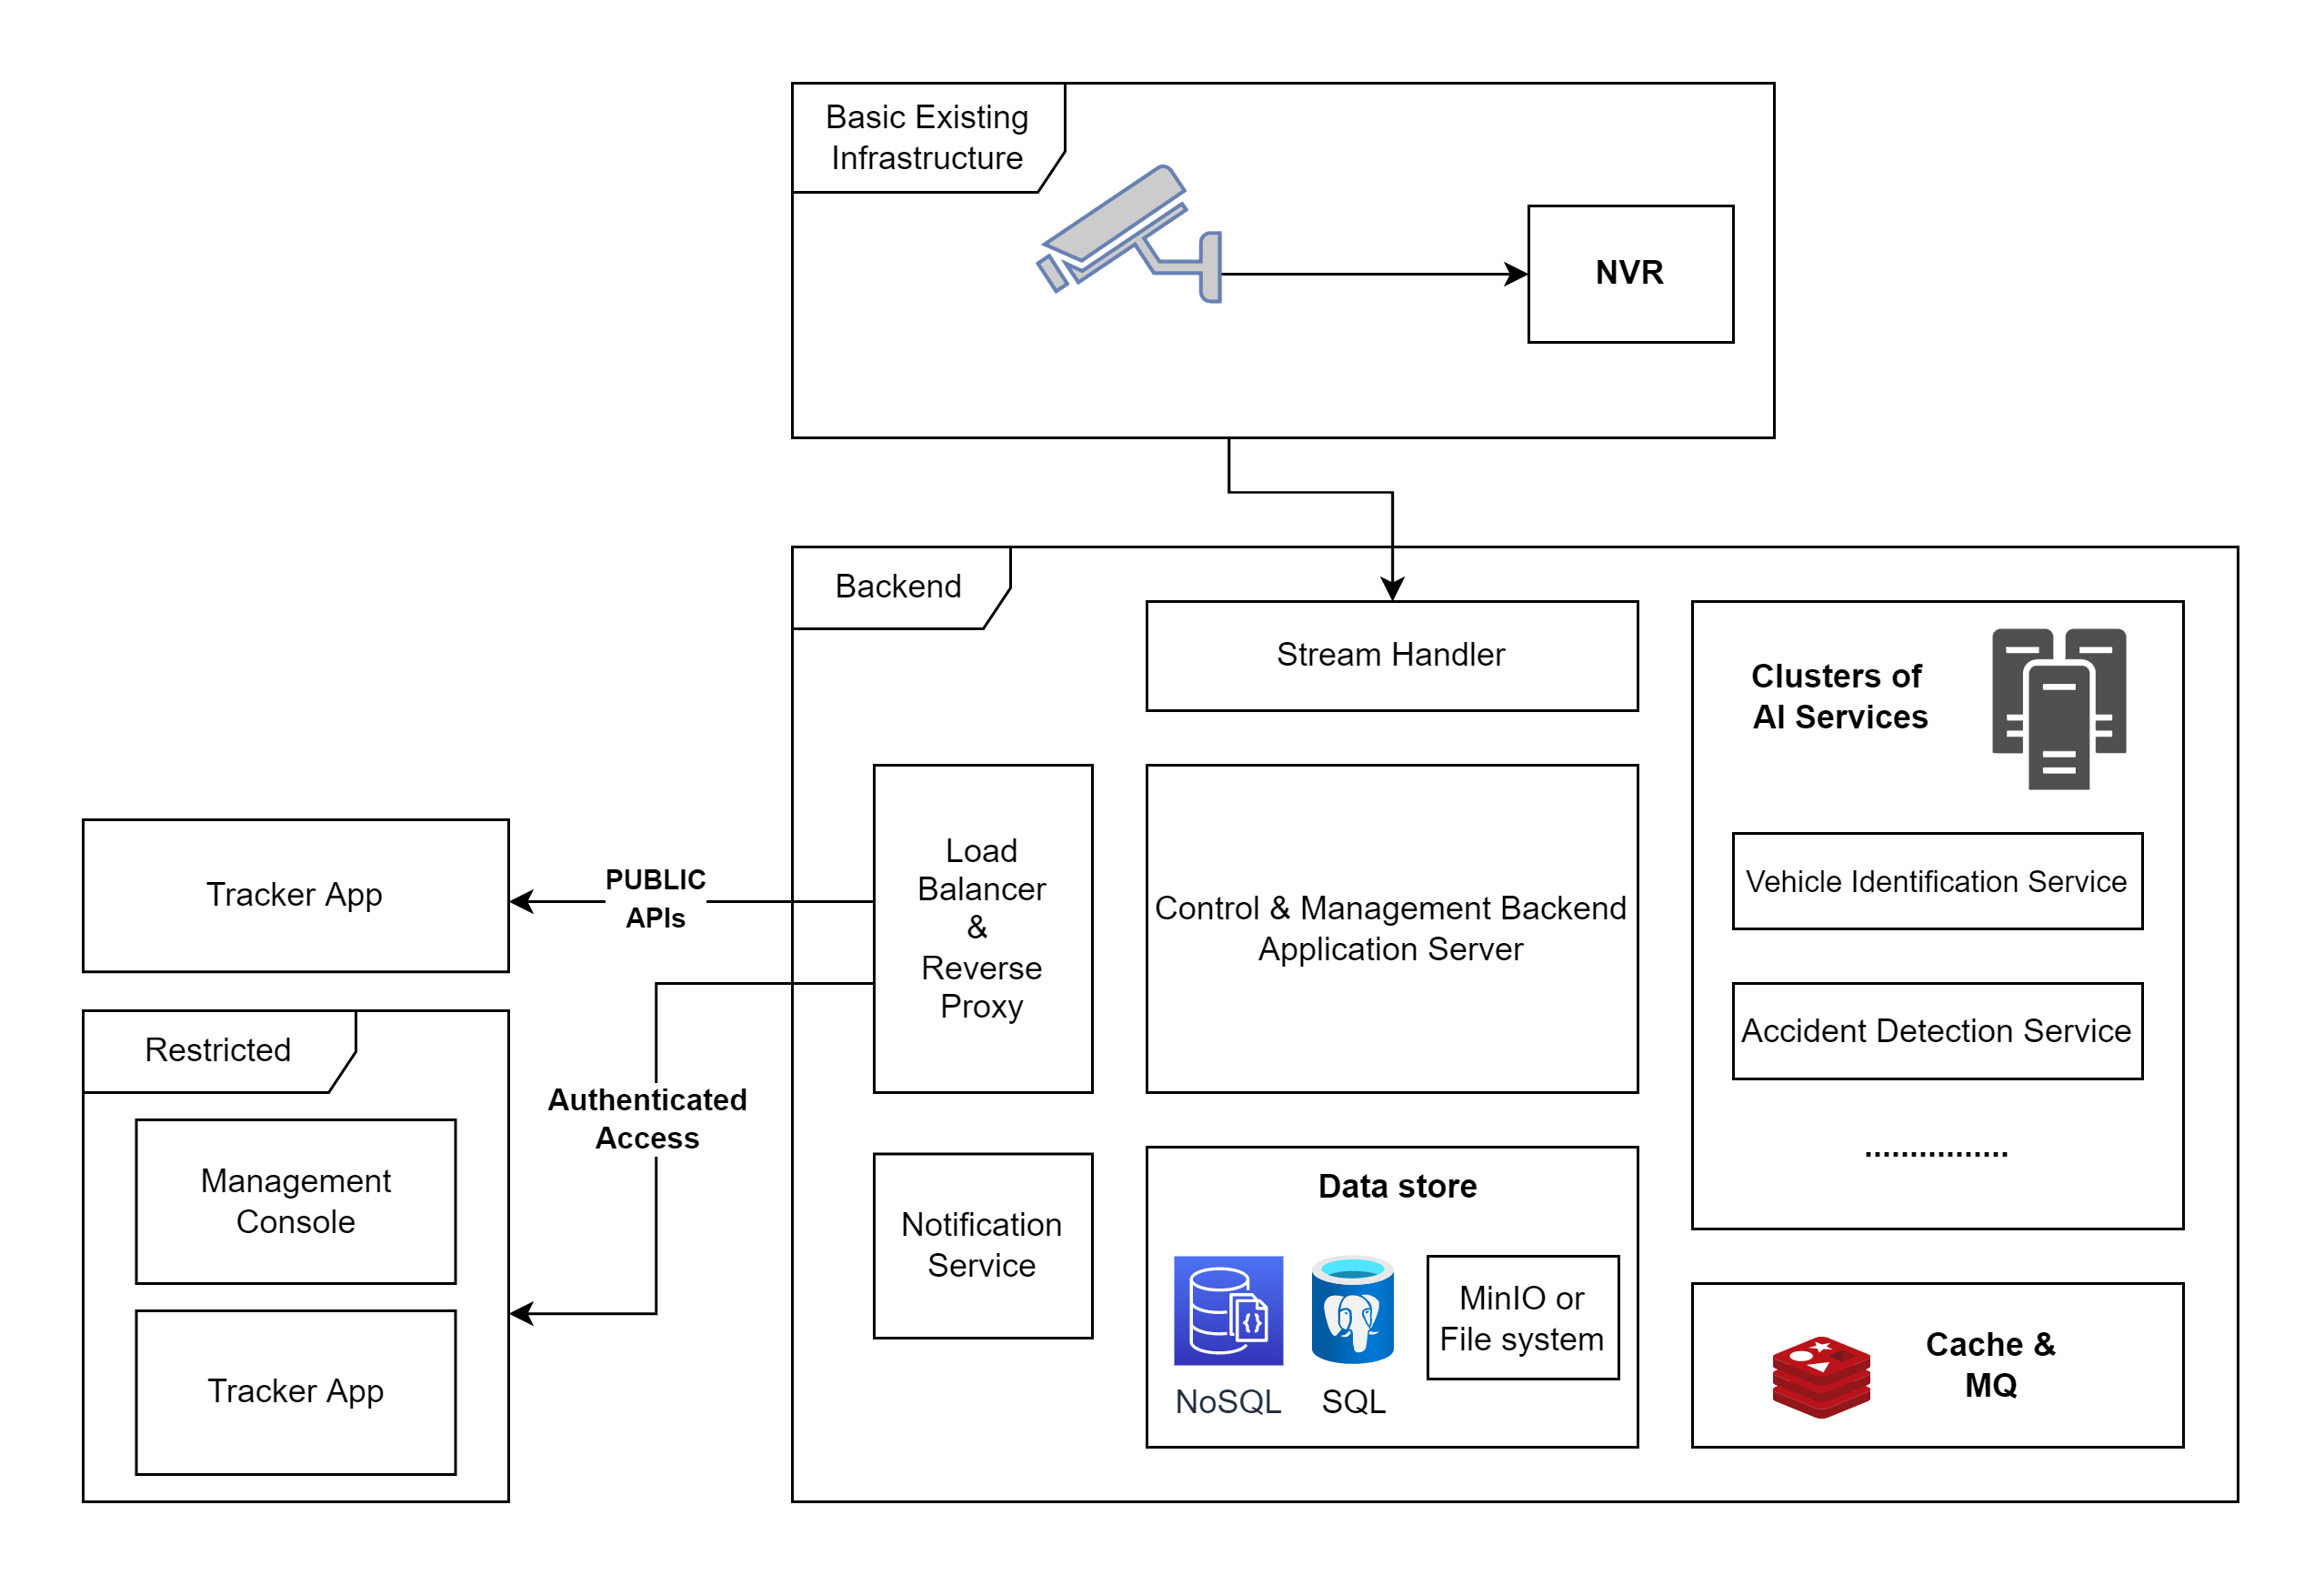
\includegraphics[width=0.8\linewidth]{Images/architecture_high_level}
	\caption{High level system architecture}
	\label{fig:architecturehighlevel}
\end{figure}

\lipsum[1-2]

\subsection{Existing CCTV Infrastructure}
Modern Infrasturcture of CCTV (Closed-Circuit Television) Video surveillance system pan out to a Network connected IP camera, which is streamed to an NVR (Network Video Recorder). Popular streaming protocols like RTSP (Realtime Streaming Protocol), RTSPS (RTSP over SSL), RTMP (Real-Time Messaging Protocol) are utlised in most IP cameras and NVR. 

NVR stores the footage and is usually removed after specificed period based on the storage capacity of the NVR and number of cameras connected. On most NVR firmares, playback and downloading of recording is only provided by builtin web interface, or propriotary softwares bundled, which are known to be poorly implemented. Some NVR interface only works with full features on outdated Internet Explorer after installing plug-in.

Live streams of NVR and IP cameras can be accessed easily as RSTP stream using the network ip address, which can be played by any client in the same network.

\subsection{VPN based Secure network access}
CCTV Video surveillance systems utlise restricted closed network isolated from the internet, to reduce cyber attack vectors and unauthorised usage. Unsecured connection and system usage can compromise the security of network. 
Constructing a VPN (Virtual Private Network) split tunnel can enable secure communication interface to the network over unsecured channels. Wiregaurd, distributed in Linux Kernel, is utlised in our design to create VPN interface with very less overhead and very high performance.


\begin{figure}
	\centering
	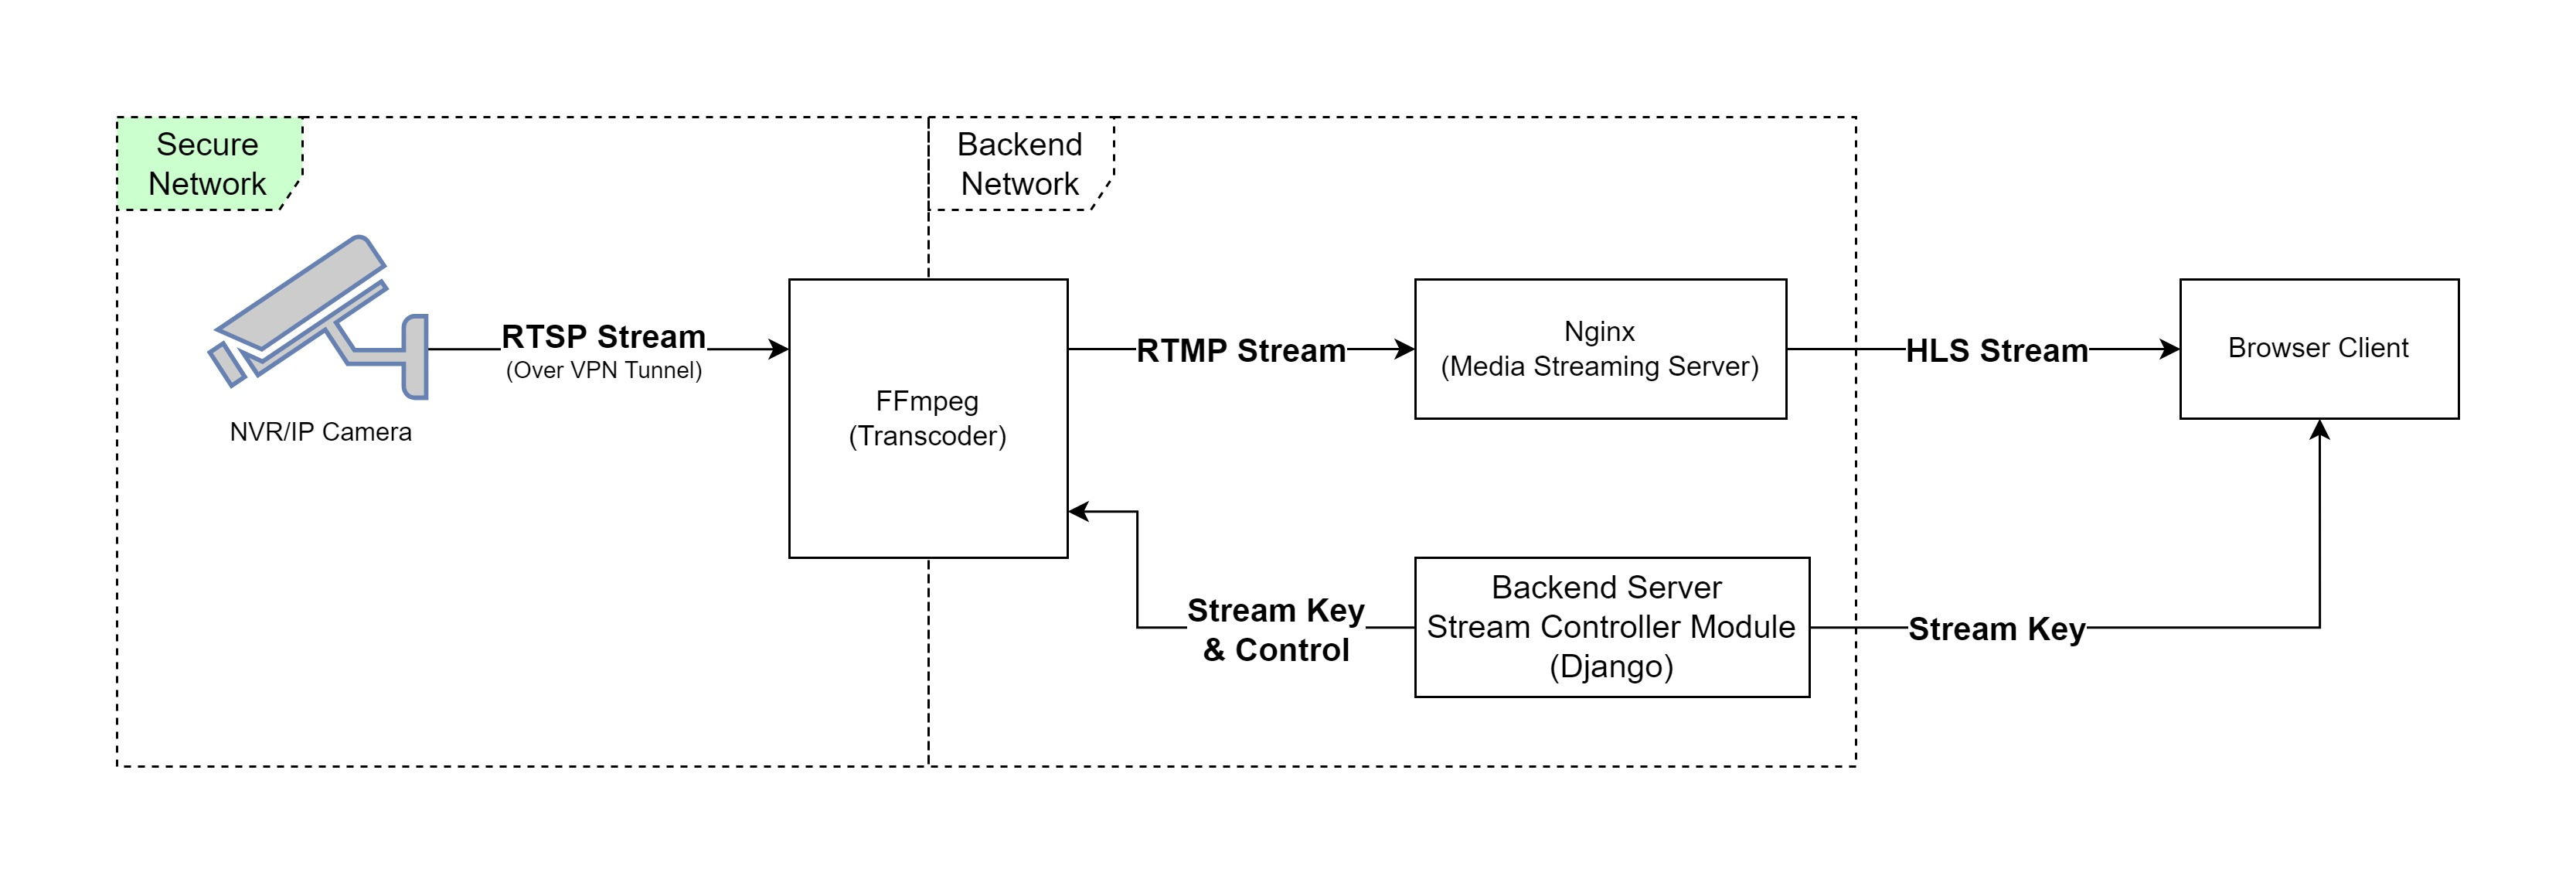
\includegraphics[width=0.8\linewidth]{Images/live_stream_arch}
	\caption{Camera Feed Live Streaming}
	\label{fig:livestreamarch}
\end{figure}

\subsection*{Technology Stack}
A hybrid microservice architecture is utlised to gain the scalability and decouple AI engine and services to serve web request efficiently, while ensuring quicker and simpler development and deployment. Each independent services are created as a separate moduluar microservice which can be integrated based on requirement and infrastructure availability.

Development is primarily done in Python, while JavaScript is utlised for frontend scripting.

The list of frameworks and libraries used represent those which are widely utlised or have significant imapact in the development.

Languages:
\begin{itemize}
	\item Python (Primary Language): Used in all serverside code.
	\item JavaScript: Used in frontend Scripting, WebSocket Browser Client, OpenPlayerJS
\end{itemize}

Frameworks:
\begin{itemize}
	\item Django: Backend Server
	\item FastAPI: AI Engine API web framework and WebSocket Abstraction
	\item TensorFlow and YOLO: AI inferencing
	\item 
\end{itemize}

Other:
\begin{itemize}
	\item Nginx: Used as web server and reverse proxy for handling request, serving static files, proxying request to application servers.
	\item Nginx RTMP Module: Used to enhance Nginx to be used as a Media Streaming Server
	\item PostgreSQL: As Relational Database
	\item Wiregaurd: Creating secured encrypted VPN tunnel to NVR infrastructure network
	\item FFmpeg: For on-the-fly video transcoding to relay Live Camera RSTP feed to nginx as RTMP ingress feed
	\item OpenCV: Image Proccessing in FrameGen module and handling camera feed.
	\item WebSocket: Bidirectional server push communication with user
	\item OpenPlayerJS: Browser-based HLS video stream playback
	\item MinIO: File and object storage backend to replicate Amazon Web Service S3.

\end{itemize}


\begin{figure}
	\centering
	\begin{subfigure}[b]{0.8\linewidth}
		\centering
		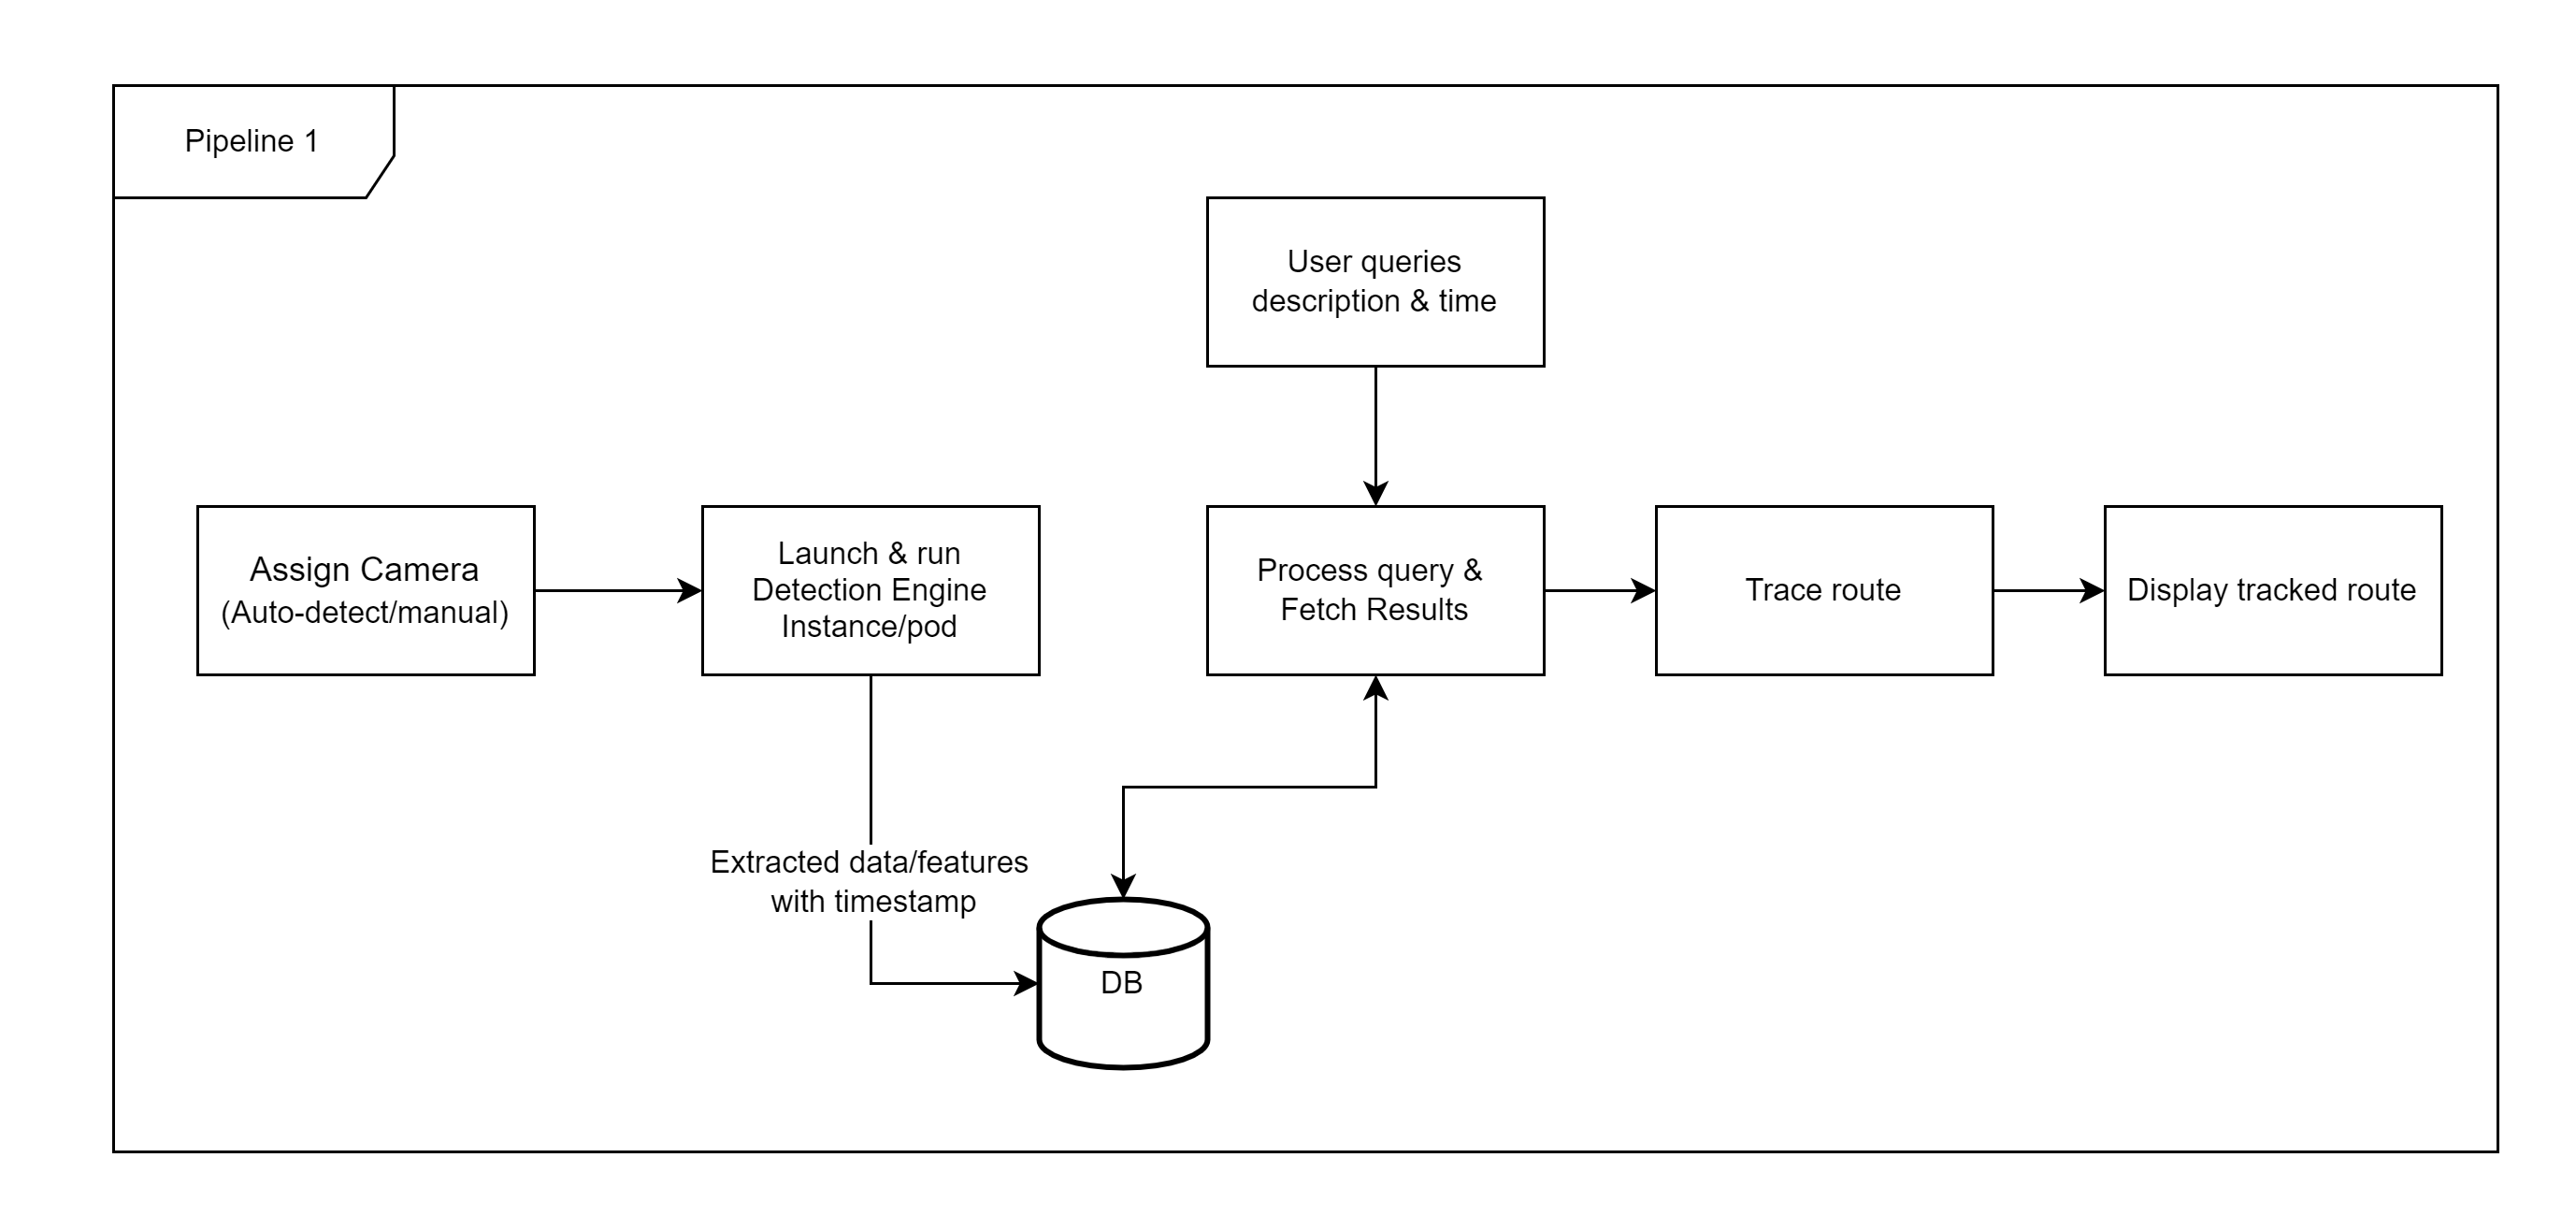
\includegraphics[width=\linewidth]{Images/pipeline1}
		\caption{pipeline1}
		\label{fig:pipeline1}
	\end{subfigure}

	\begin{subfigure}[b]{0.8\linewidth}
		\centering
		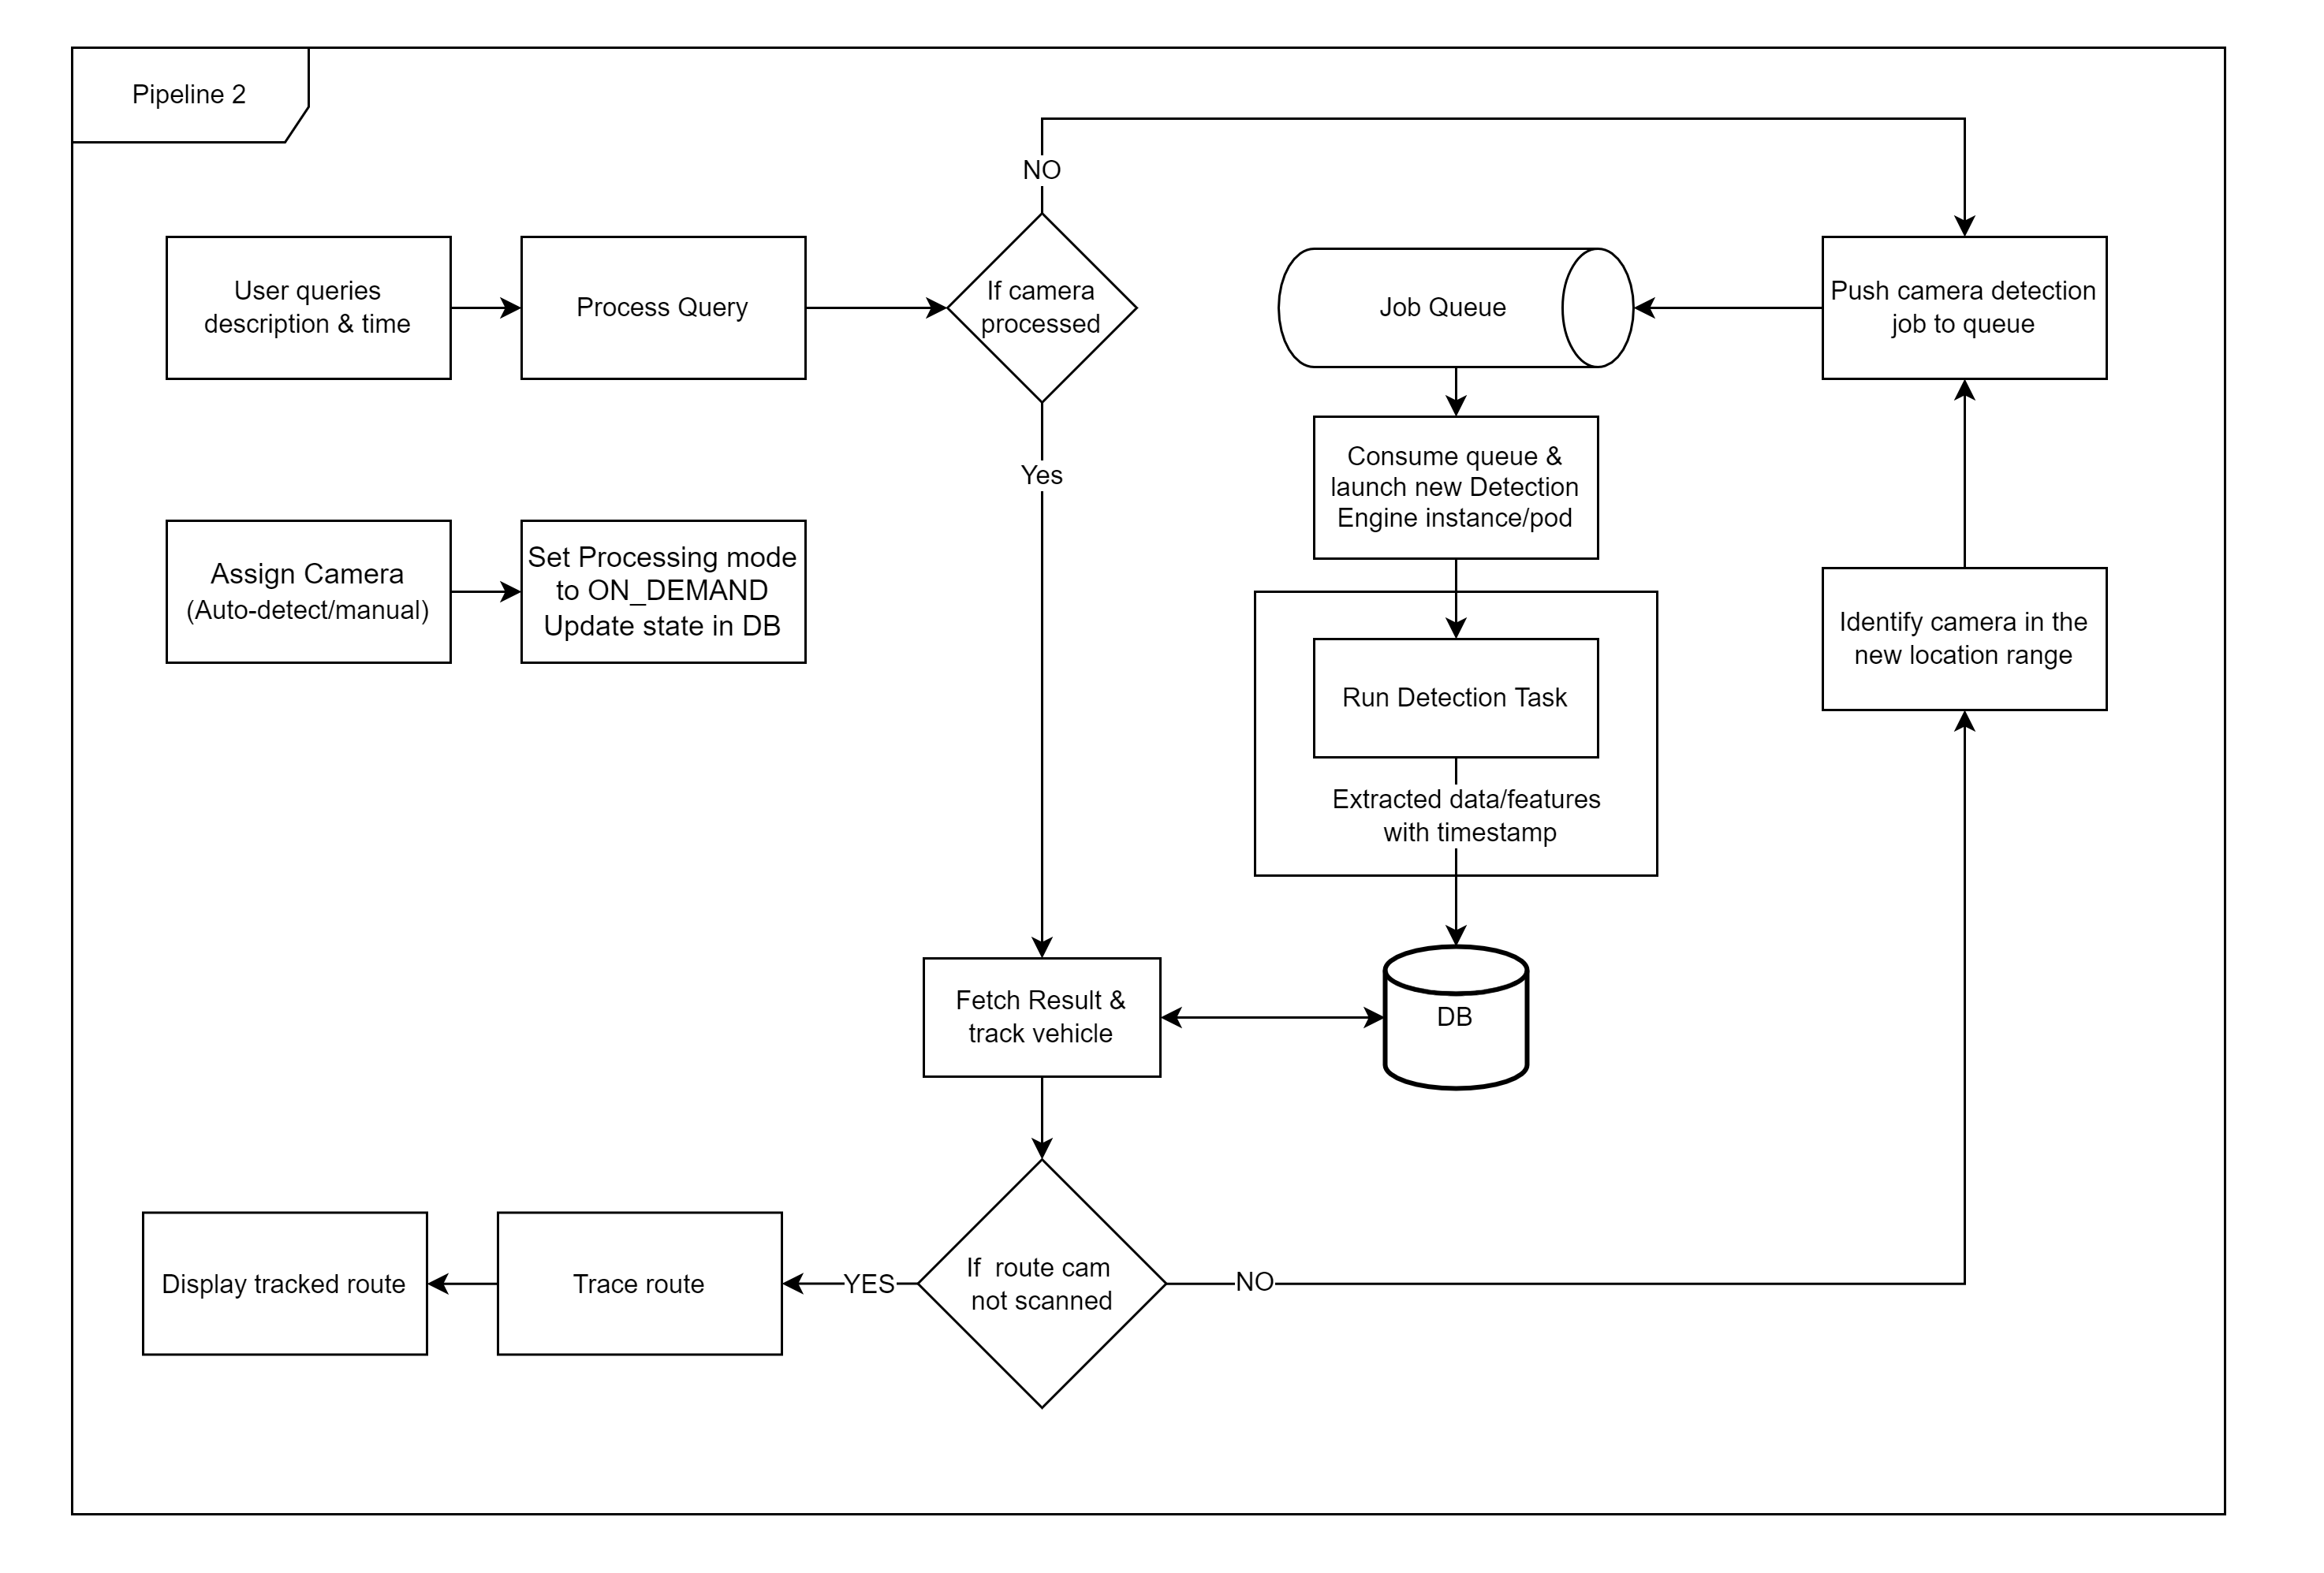
\includegraphics[width=\linewidth]{Images/pipeline2}
		\caption{pipeline2}
		\label{fig:pipeline2}
	\end{subfigure}
	\caption{Workflow pipeline}
\end{figure}

\lipsum[1-2]
 


\section{Camera Network}
The camera feed is obtained from a project deployed by Center for Information, Communication and Educational Technology (CICET), Government College of Engineering Kannur. Under the project entitled "Third eye", a virtual network was established covering an area of 350 $KM^2$, connecting 9 institutes. Using the existing cable network, various camera at installed allowing easy and secure storage and streaming. Currently the project houses holds about 190 cameras. Excess to these footage if obtained by secured virtual private junction.

\begin{figure}[!ht]
	\centering
	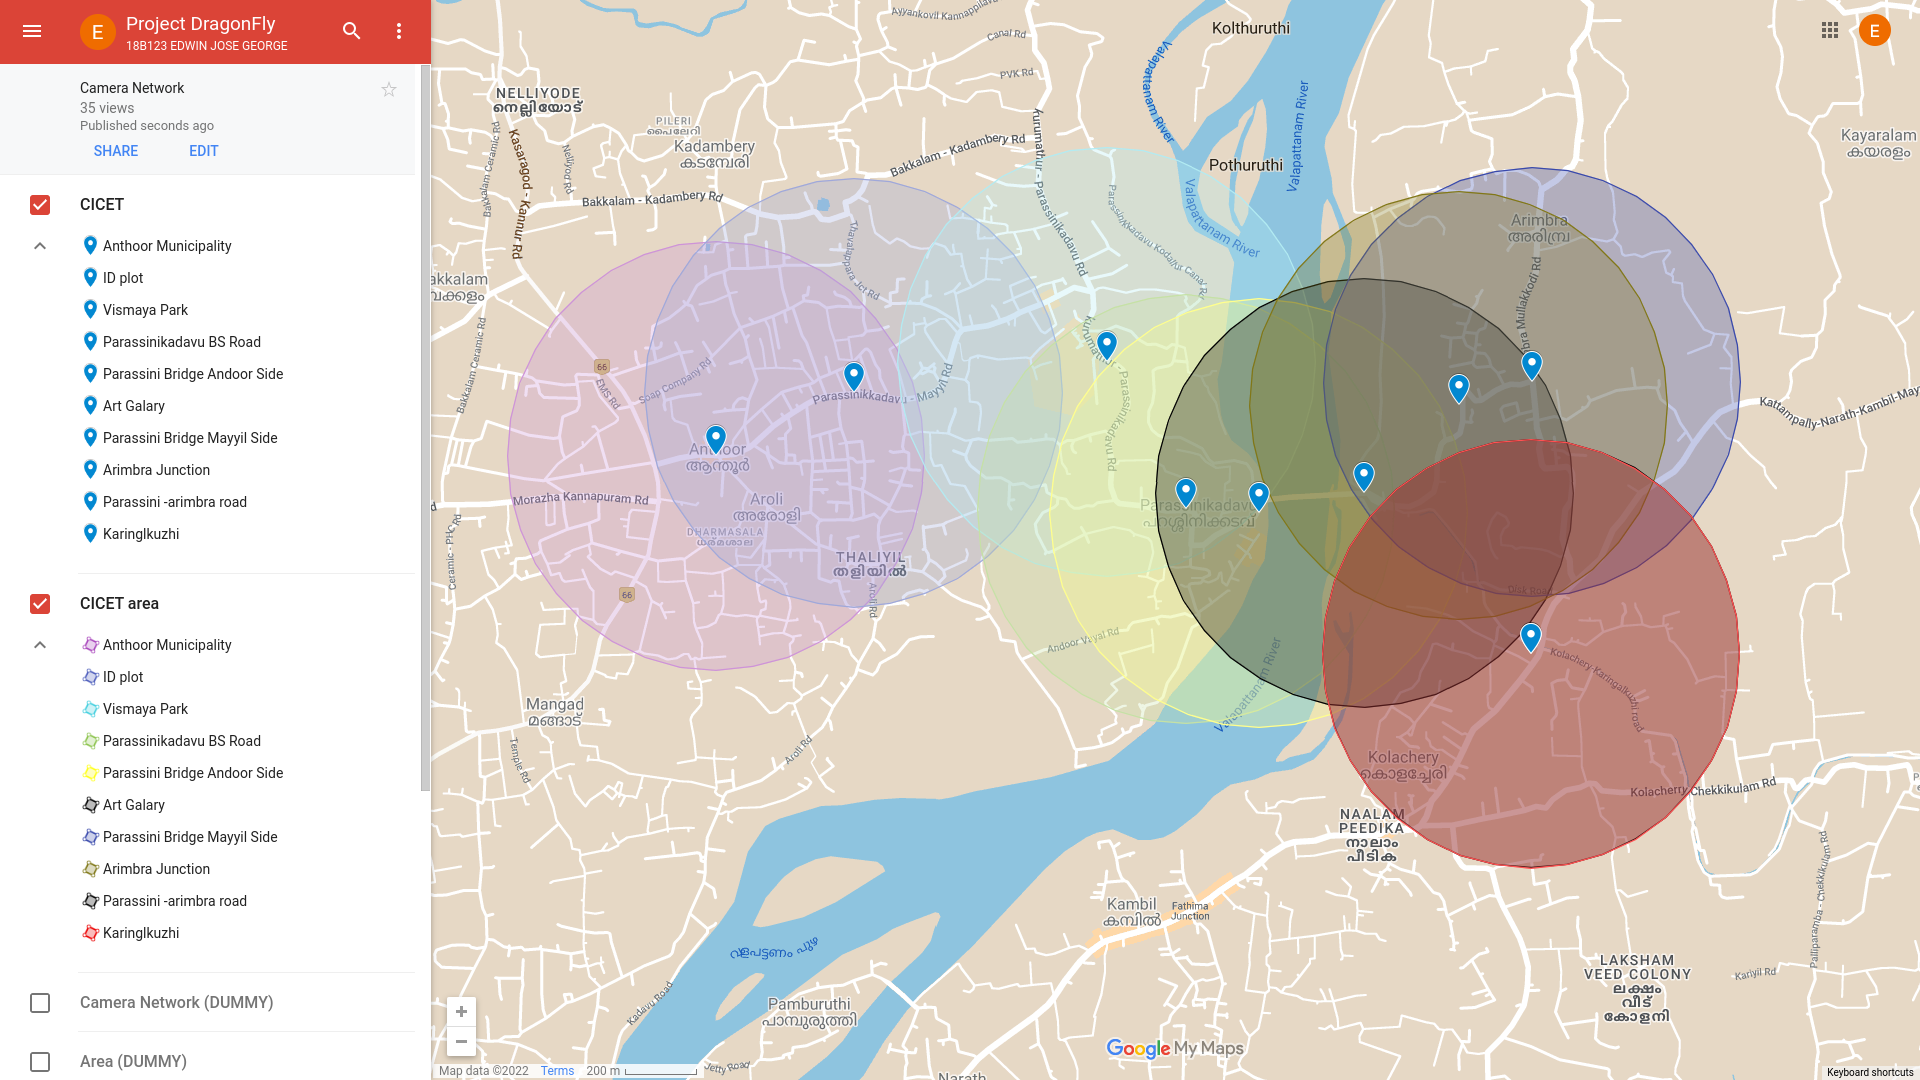
\includegraphics[width=\linewidth]{Images/camera-network}
	\caption{CICET camera network}
	\label{fig:camera-network}
\end{figure}

\begin{figure}[!ht]
	\centering
	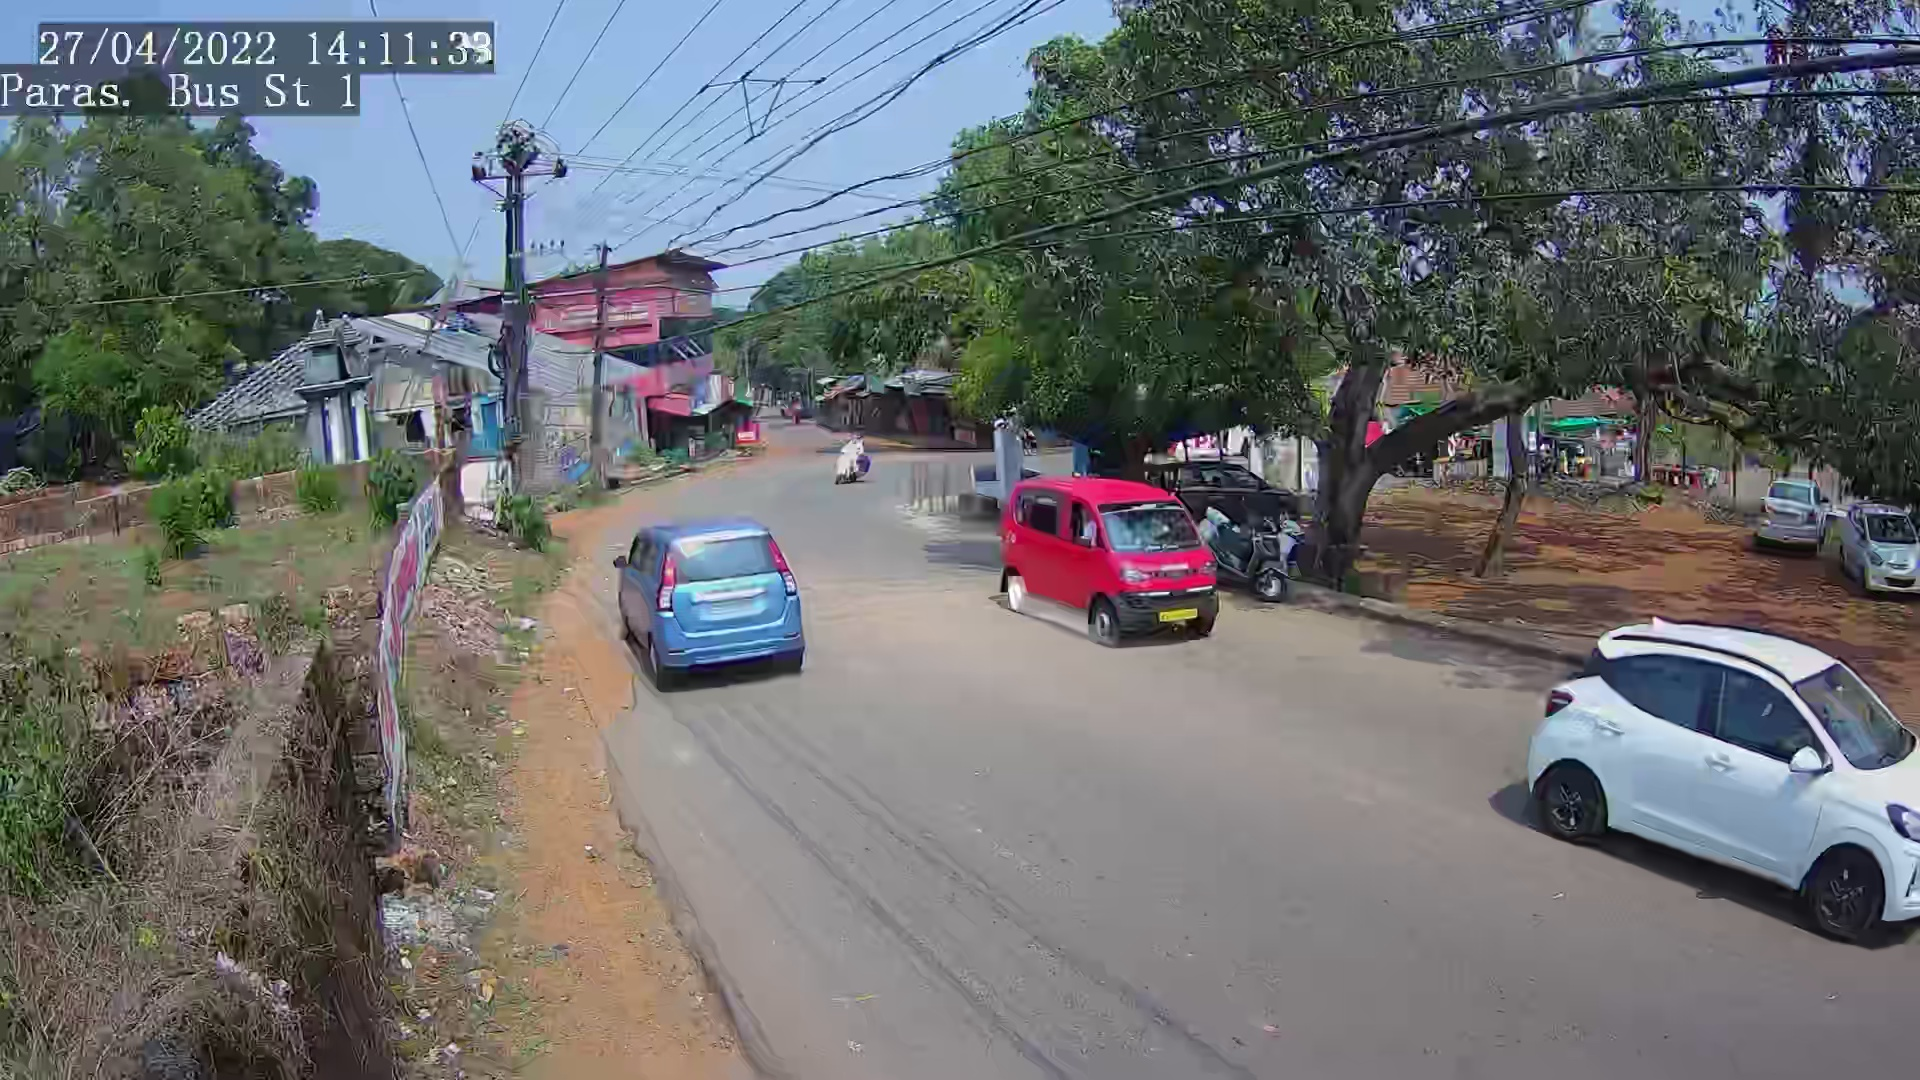
\includegraphics[width=0.32\linewidth]{Images/camera_footage/footage1} \hfill
	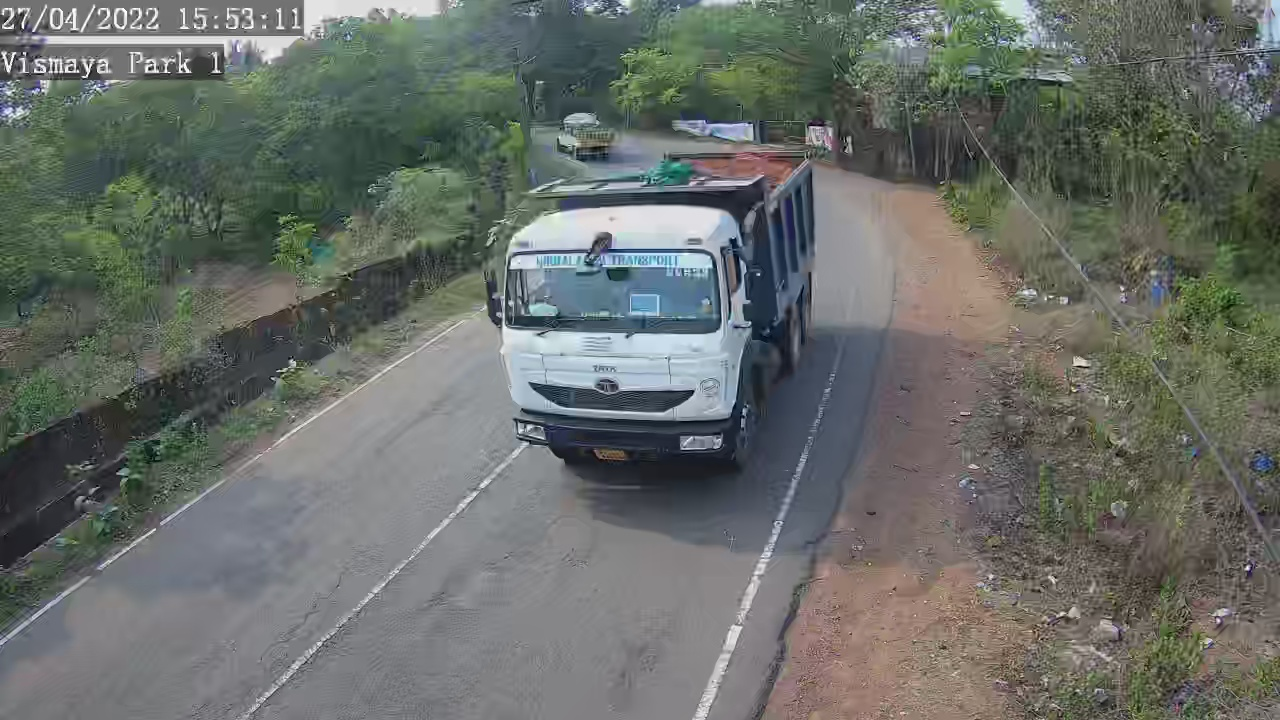
\includegraphics[width=0.32\linewidth]{Images/camera_footage/footage2} \hfill
%	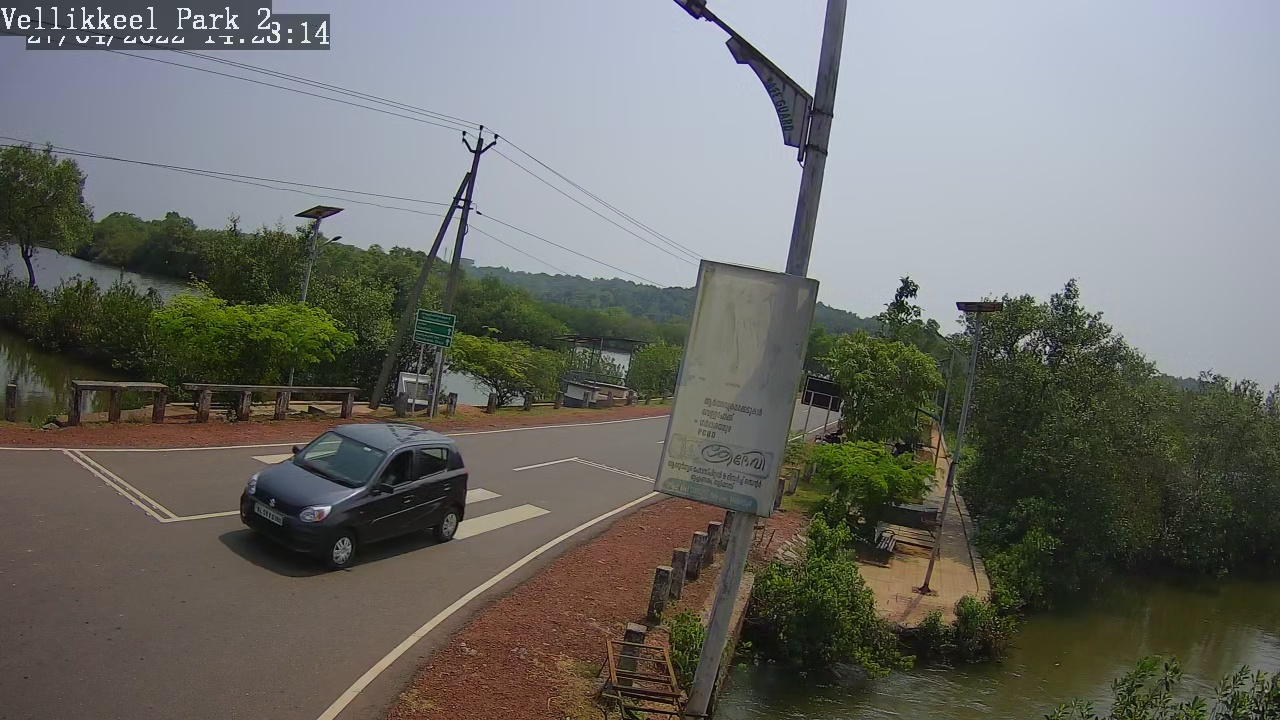
\includegraphics[width=0.32\linewidth]{Images/camera_footage/footage3} \\
%	\vspace{3mm}
%	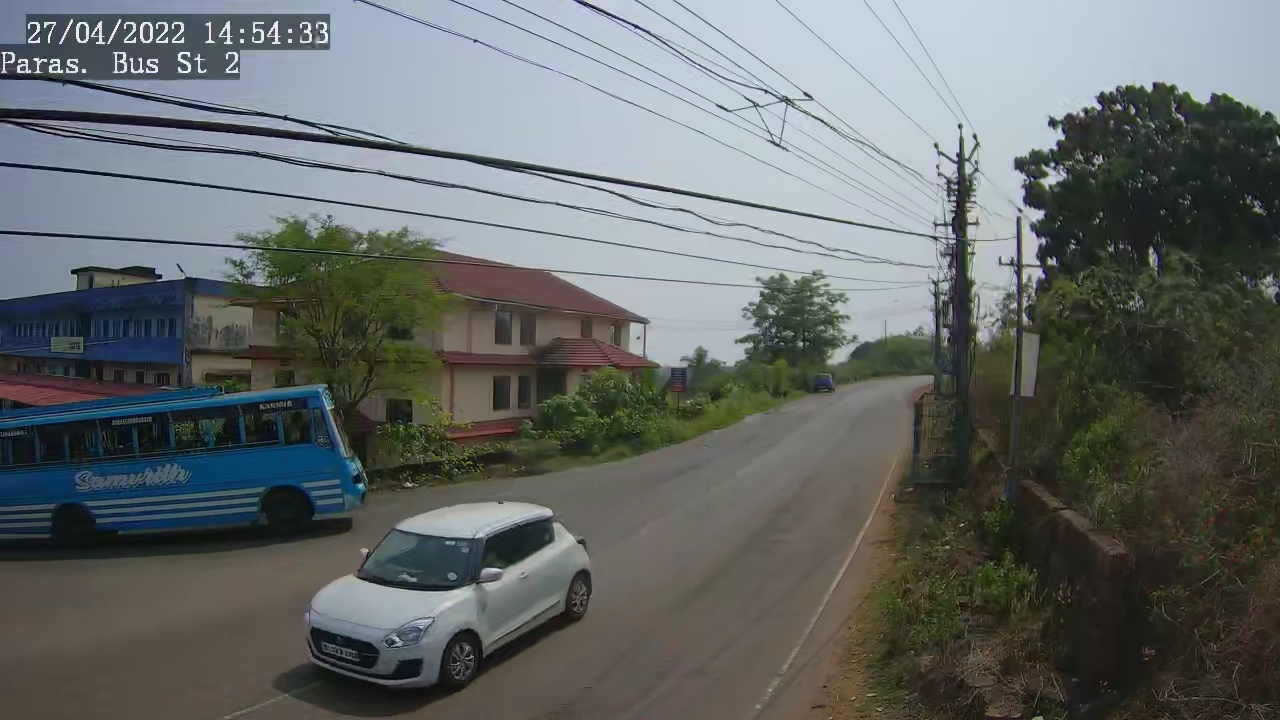
\includegraphics[width=0.32\linewidth]{Images/camera_footage/footage4} \hfill
	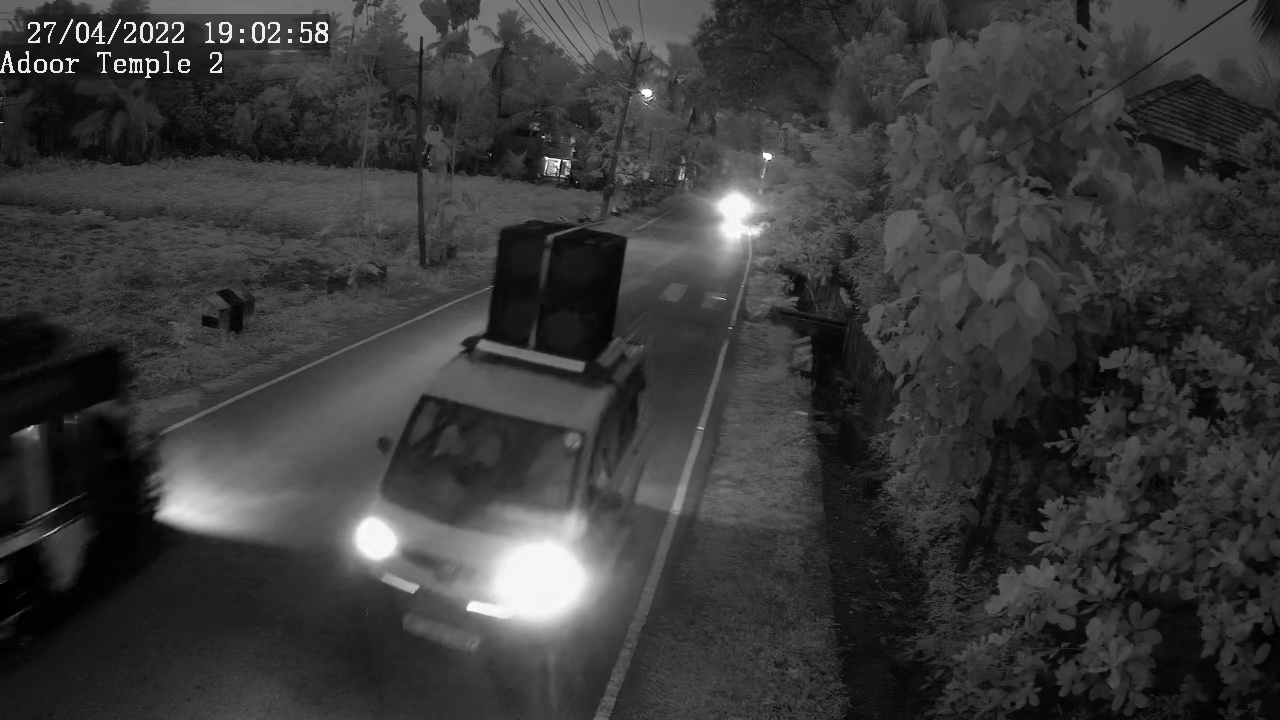
\includegraphics[width=0.32\linewidth]{Images/camera_footage/night1} \hfill
%	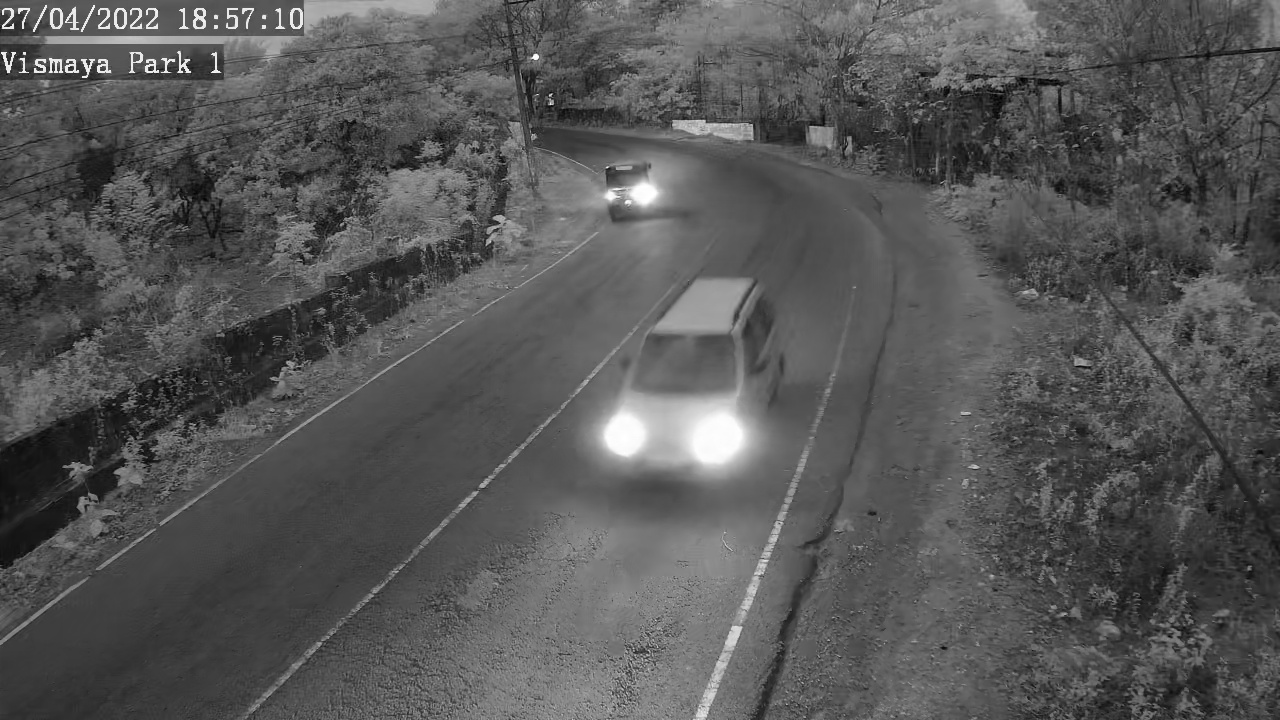
\includegraphics[width=0.32\linewidth]{Images/camera_footage/night2}
	\caption{Sample camera footage}
\end{figure}


\section{UI Design}

\lipsum[1]

\begin{figure}[!ht]
	\centering
	\begin{subfigure}[b]{0.48\linewidth}
		\centering
		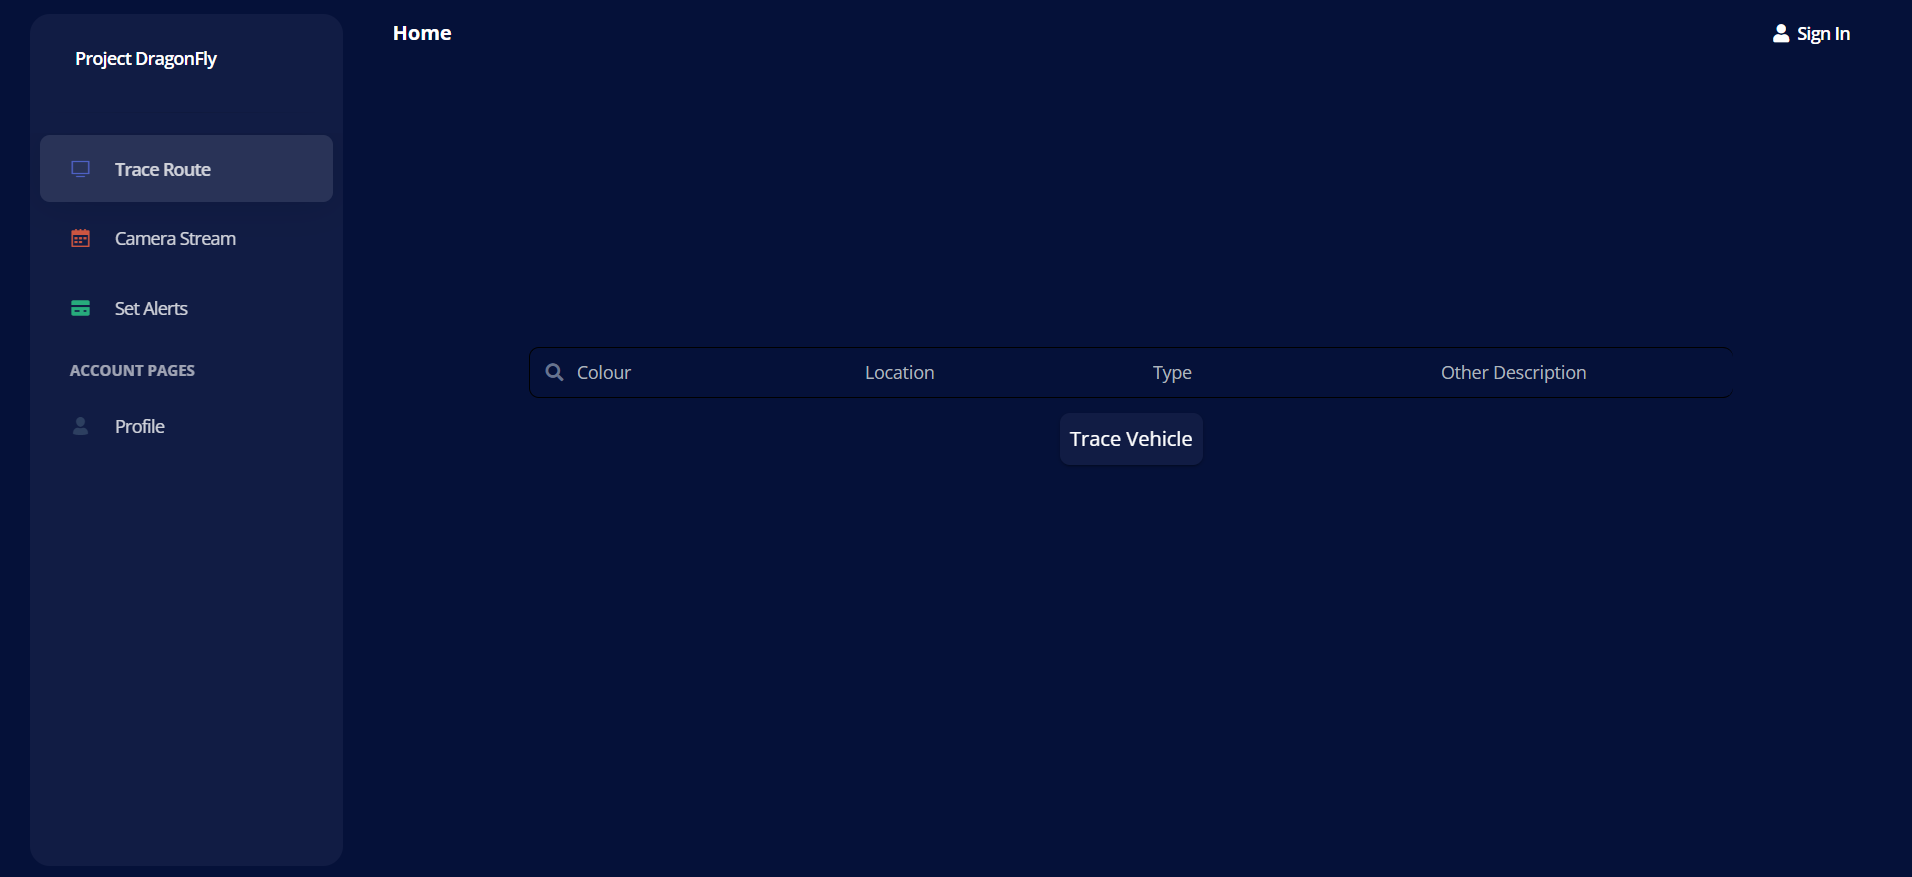
\includegraphics[width=\linewidth]{Images/UI/home}
		\caption{Home page}
		\label{fig:home}
	\end{subfigure} \hfill
	\begin{subfigure}[b]{0.48\linewidth}
		\centering
		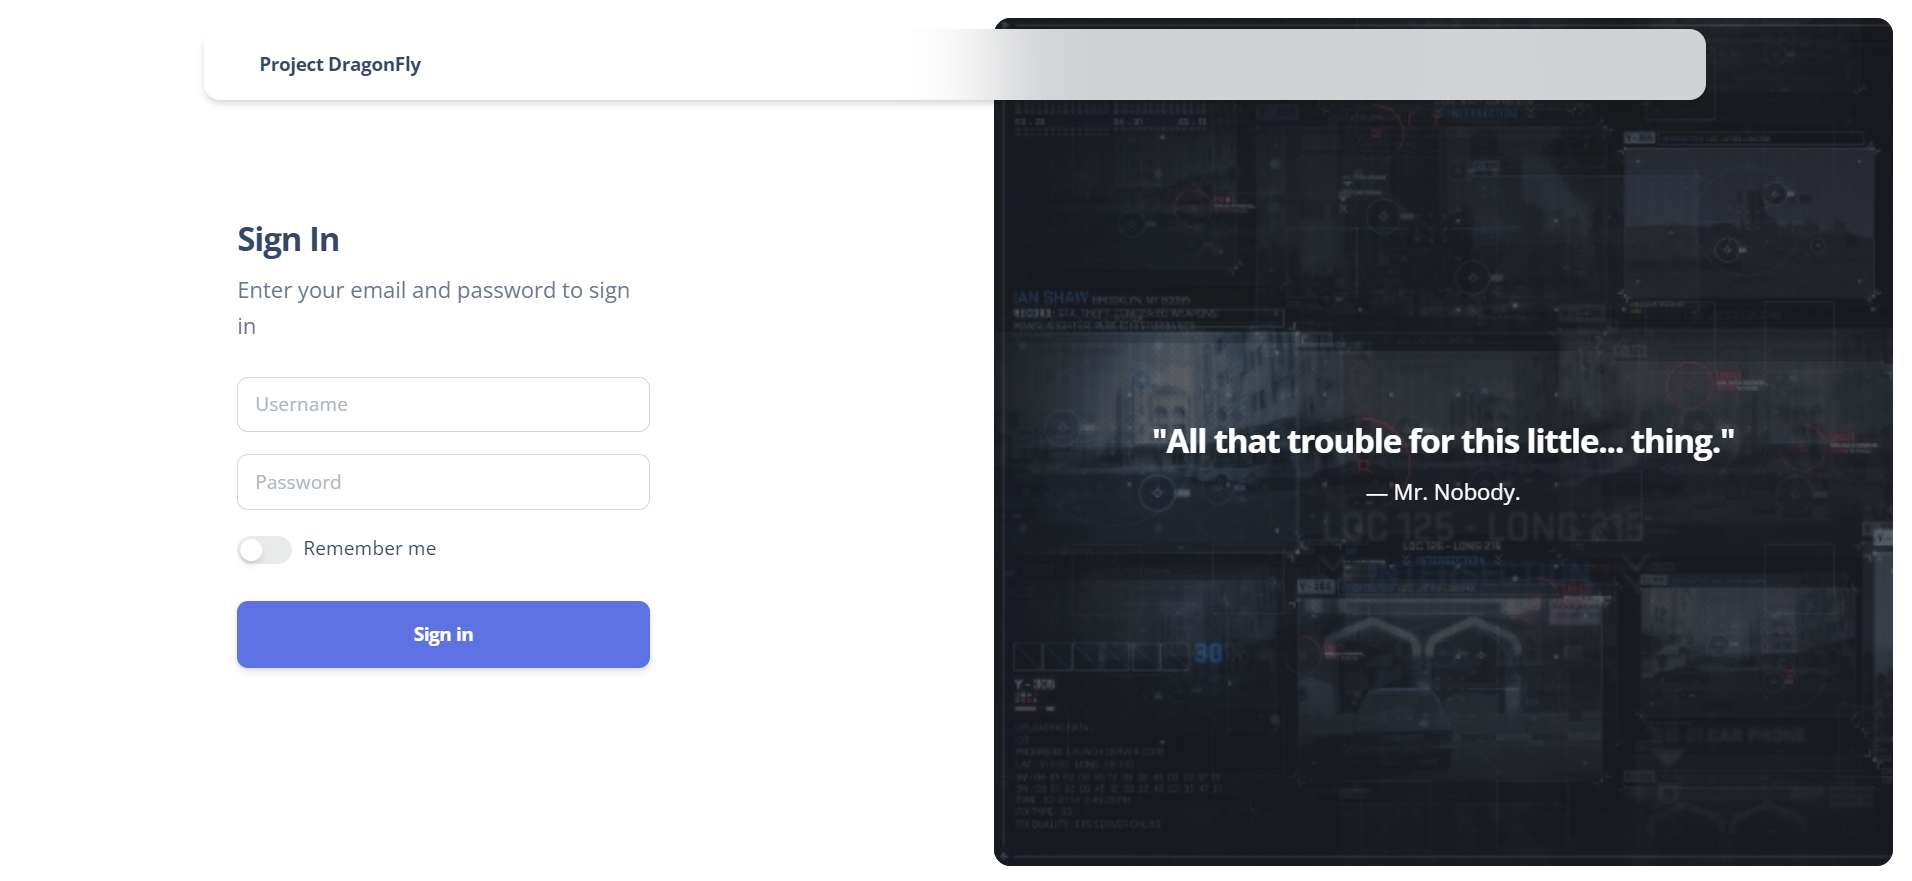
\includegraphics[width=\linewidth]{Images/UI/login}
		\caption{Login page}
		\label{fig:login}
	\end{subfigure} \\ \vspace{3mm}
	\begin{subfigure}[b]{0.48\linewidth}
		\centering
		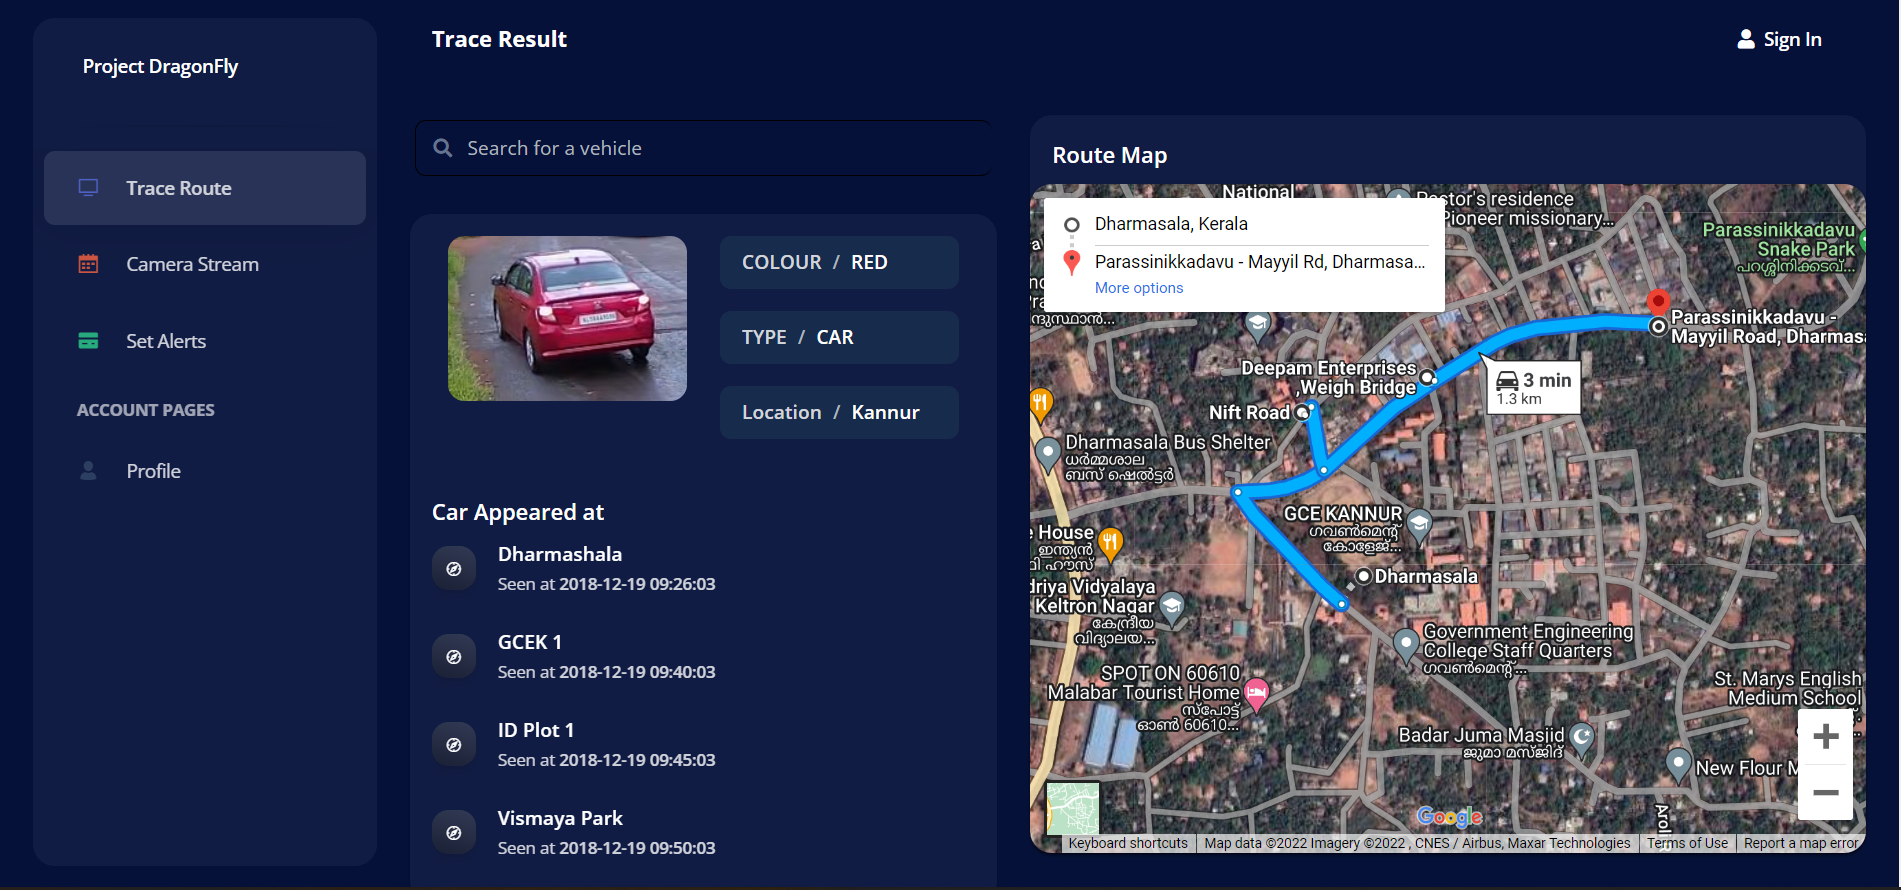
\includegraphics[width=\linewidth]{Images/UI/result}
		\caption{Result}
		\label{fig:result}
	\end{subfigure} \hfill
	\begin{subfigure}[b]{0.48\linewidth}
		\centering
		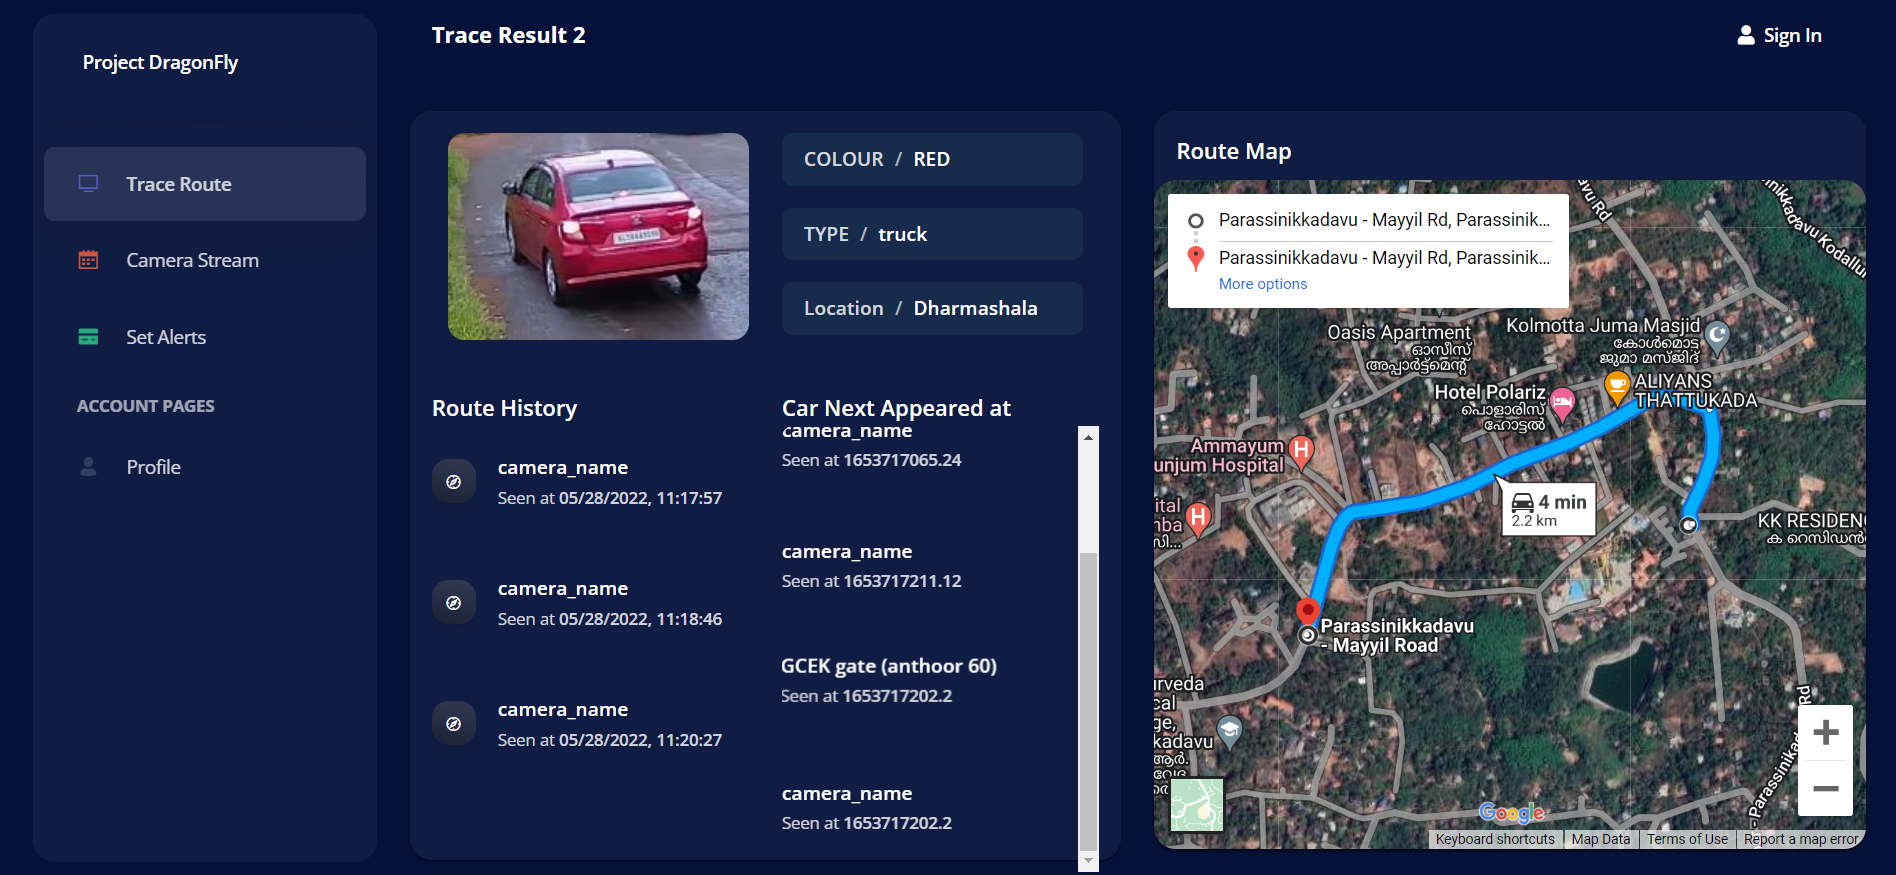
\includegraphics[width=\linewidth]{Images/UI/tracing}
		\caption{Tracing}
		\label{fig:tracing}
	\end{subfigure}
	\caption{UI Design}
\end{figure}

\lipsum[1]

\section{AI Model}
\subsection*{YOLOv4}
YOLOv4 model is used for the detection of vehicles. Transfer learning was conducted on the AI model that significantly reduced the training time required. Transfer learning is the process of using a pre-trained model and changing its parameter to learn new/fine tuned concept. Pre-trained weight was extracted from the official YOLOv4 repository \cite{darknet} that used MS COCO dataset to train 80 classes. Parameter tuning is performed which are detailed in table \ref{tab:yolo_parameter}.

\begin{table}[!ht]
	\centering
	\begin{tabular}{|l|l|}
		\hline
		Input size            & $416 * 416$  \\ \hline
		Input Channels        & 3            \\ \hline
		Batch size            & 32           \\ \hline
		learning rate         & 0.0013       \\ \hline
		Yolo layer            & $[256*256],[512*512],[1024*1024]$ \\ \hline
		Total Layers          & 162          \\ \hline
		Target Classes (9)    & \begin{tabular}[c]{@{}l@{}}
			auto, bus, tempo traveler, tractor, \\
			truck, van, two wheeler, car, jcb\end{tabular} \\ \hline
	\end{tabular}%
	\caption{YOLOv4 Parameter}
	\label{tab:yolo_parameter}
\end{table}

The model was trained using Darknet at Google Colab. Later the environment was changed to the Workstation provided by the Dept. of Computer Science and Engineering, Govt. College of Engineering Kannur. A total of approx. 48 hours are spend in training, reaching 97.7\% mean Average Precision (mAP) at 7300 iterations. Figure \ref{fig:darknettrainingchart} summarizes training.

The dataset for training was collected at two different sources. Kaggle provided a wide variety of Indian Vehicle dataset that spanned across country. Footage from CICET camera network is also extracted. Each and every frame was labeled using LabelImg tool. Summary of the labeled dataset is depicted in the table \ref{tab:dataset_sum1}.

\begin{table}[!ht]
	\begin{tabular}{m{0.45\linewidth} m{0.45\linewidth}}
%		\begin{figure}
			\centering
			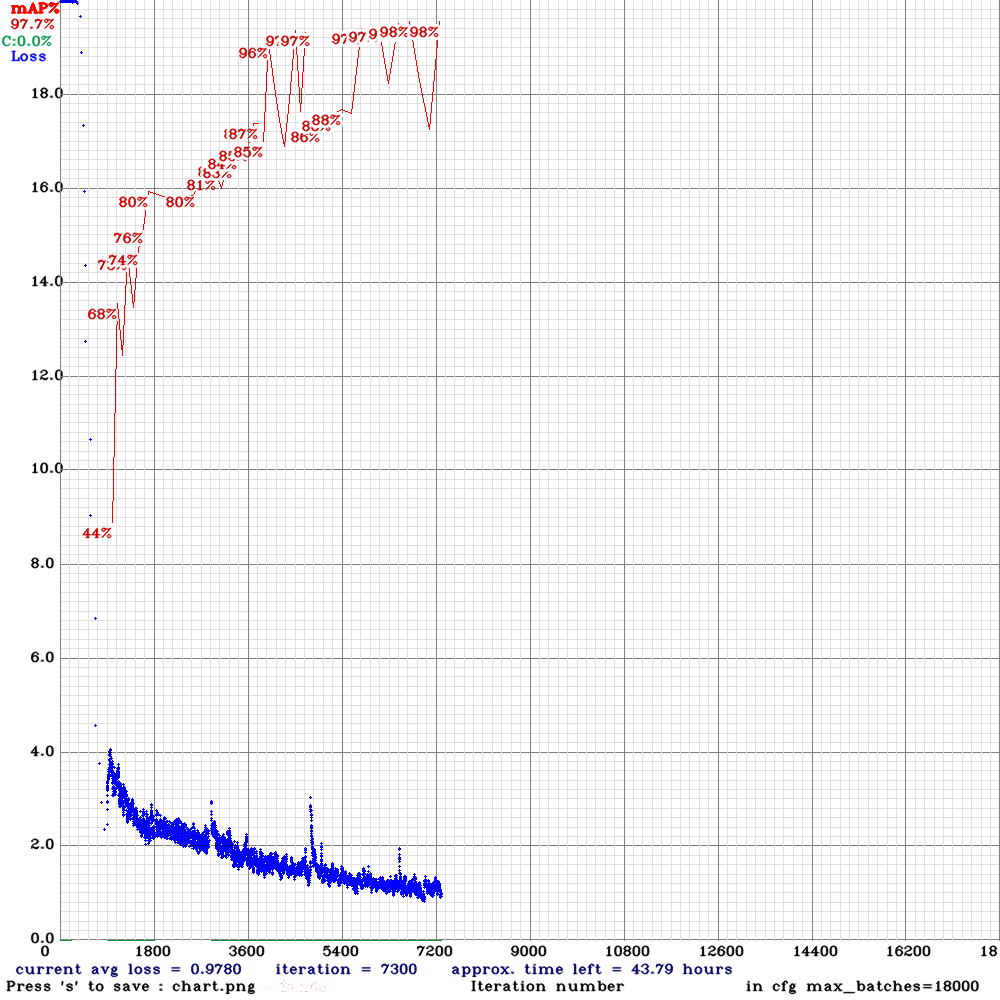
\includegraphics[width=\linewidth]{Images/darknet_training_chart}
			\captionof{figure}{YOLOv4 training chart}
			\label{fig:darknettrainingchart}			
%		\end{figure}

		 & 
		 
		 \begin{tabular}{|l|c|c||c|}
		 	\hline
		 	\textbf{Class}        & \textbf{Kaggle} & \textbf{CICET} & \textbf{Total} \\ \hline
		 	Two wheeler           & 557             & 291            & \textbf{848}   \\ \hline
		 	Truck                 & 354             & 170            & \textbf{424}   \\ \hline
		 	Auto                  & 297             & 146            & \textbf{443}   \\ \hline
		 	car                   & 233             & 432            & \textbf{665}   \\ \hline
		 	bus                   & 220             & 112            & \textbf{332}   \\ \hline
		 	tractor               & 133             & 0              & \textbf{113}   \\ \hline
		 	van                   & 101             & 131            & \textbf{232}   \\ \hline
		 	JCB                   & 1               & 0              & \textbf{1}     \\ \hline \hline
		 	\textbf{Total Boxes}  & \textbf{1956}   & \textbf{1282}  & \textbf{3238}  \\ \hline
		 	\textbf{Total Images} & \textbf{733}    & \textbf{826}   & \textbf{1559}  \\ \hline
		 \end{tabular}
		 \captionof{table}{Dataset summary}
		 \label{tab:dataset_sum1}
	\end{tabular}
\end{table}

\subsection*{DeepSORT}
DeepSORT is utilized to assign unique id to each object in an continuous frame. The implementation is directly extracted from the article of AIGuysCode \cite{theaiguyscode_deepsort}. The given model tries to extract human features as the deep matrix. No modification are made as Kalman filter provides greater accuracy. However, learning the deep matrix of vehicles can further increase accuracy and aid in siamese network.

\subsection{Image Dictionary}
In-order to facilitate correct labeling of images, a concept called Image Dictionary is introduced. Image Dictionary is a hierarchical classification of images. Each type can have its sub-type. A visual representation is also provided for each type. It is build using D3 JS.
\begin{figure}[!ht]
	\centering
	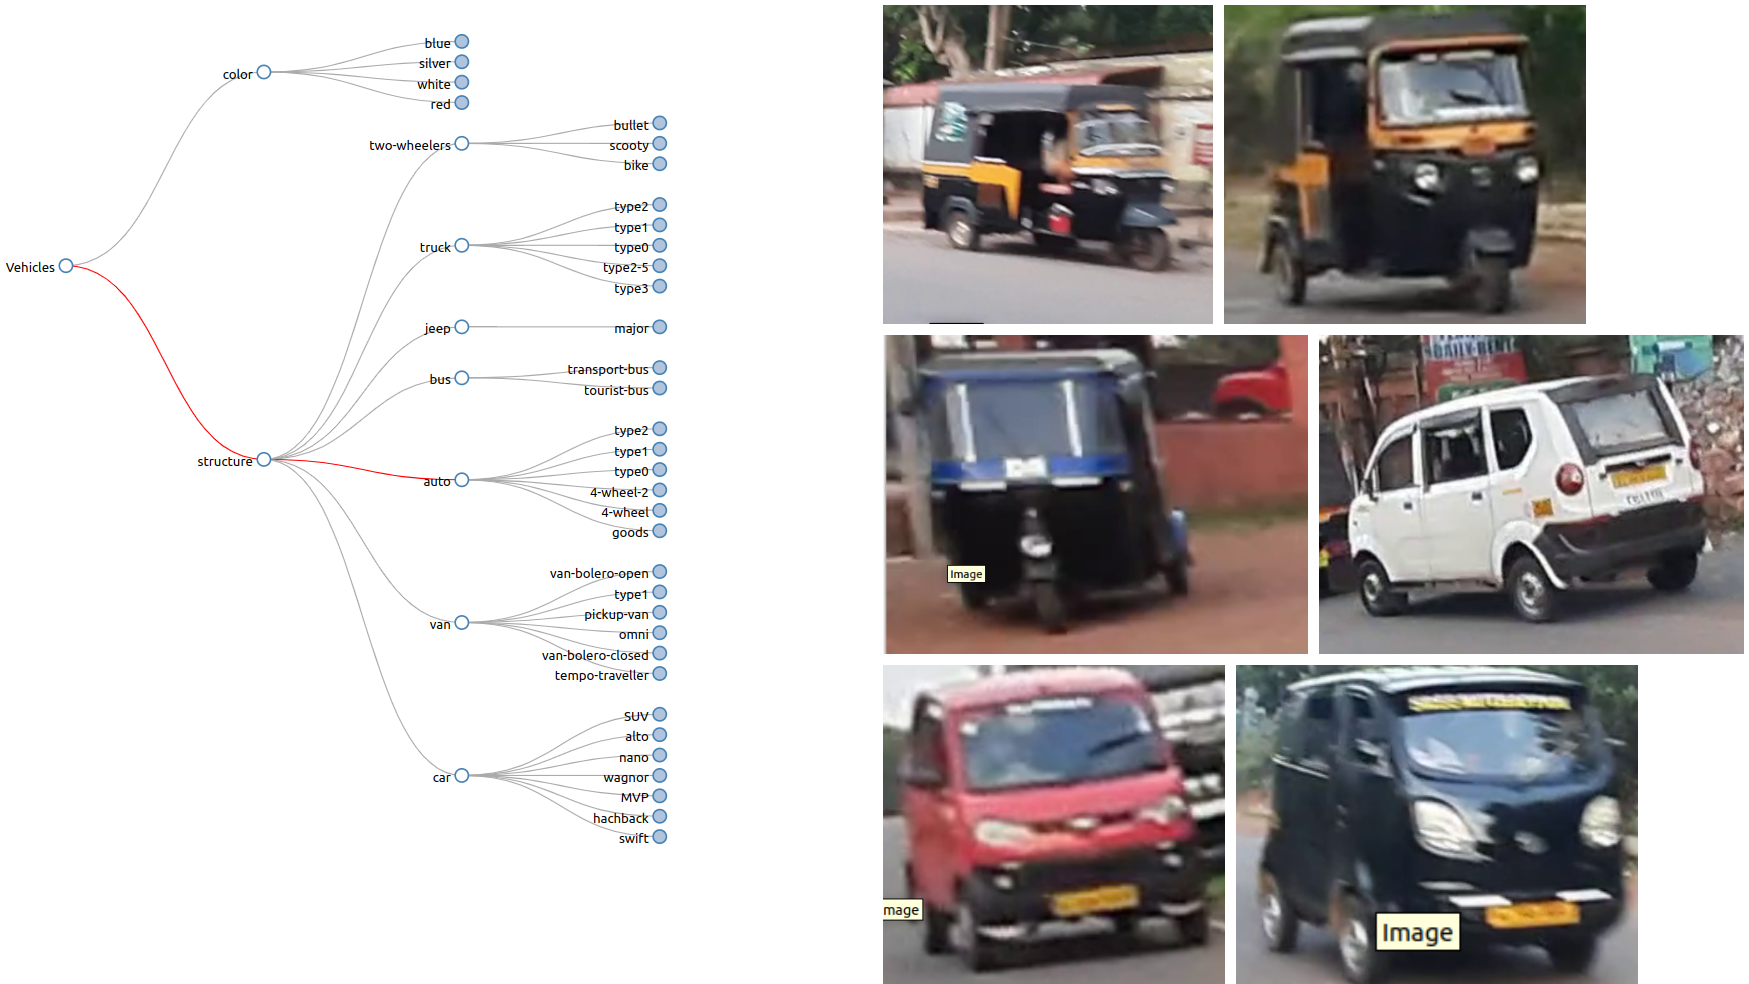
\includegraphics[width=\linewidth]{Images/image_dictionary}
	\caption{Image Dictionary}
\end{figure}


\section{Algorithm}
\begin{breakablealgorithm}
	\caption{Process and store detections $\forall$ camera}
	~~ \\\textbf{INPUT} : $video$, $camProp$
	\\ \textbf{OUTPUT} : $id$, $class$, $bbox$, $time$, $featureTensor$ $\rightarrow$ $Database$
	\begin{algorithmic}[1]
		\State $FPS \gets video.FPS$
		\State $time \gets camProp.startTime$
		\State $tracker \gets \Call{Tracker}{cosineMetric}$
		\ForAll{$frame \in video.frames$}
			\State $names, bboxes, scores \gets \Call{YOLOv4}{frame}$
			\State $features \gets \Call{encoder}{frame,bboxes}$ \Comment{feature extraction}
			\State $detections \gets []$
			\For{$i \in \Call{lenght}{names}$}
				\State $detections[i] \gets (names[i],bboxes[i],scores[i],features[i])$
			\EndFor
			\State $\Call{tracker.predict}{\space}$
			\State $\Call{tracker.update}{detections}$ \Comment{DeepSORT assigns id}
			
			\ForAll{$track \in tracker.tracks$}
				\If{$not \Call{track.isConfirmed}{\space}$} \Comment{Skip first few frame to ensure objects presence}
					\State Continue
				\ElsIf{$track.time_since_update \ge 1$} \Comment{Missing object in current frame}
					\State Continue
				\EndIf
				\State $\Call{Database.Write}{track.id, track.class, track.tbwh, time, track.feature}$
			\EndFor
			\State $time \gets time + \frac{1}{FPS}$
		\EndFor
	\end{algorithmic}
\end{breakablealgorithm}

\begin{breakablealgorithm}
	\caption{Route building}
	~~ \\\textbf{INPUT} : $vehicleClass$, $initialCamera$, $startTime$, $endTime$
	\\ \textbf{OUTPUT} : $route$
	\begin{algorithmic}[1]	
		\State $terminate \gets FALSE$
		\State $route \gets []$
		\State $vehicleList \gets []$
		\State $currentCam \gets initialCamera$
		
		\State $DB \gets currentCam.DataBase$  \Comment{Find the vehicle}
		\State $DB \gets \Call{DB.filter}{name=vehicleClass}$
		\State $fDB \gets \Call{DB.filter}{time \geq startTime}$
		\State $fDB \gets \Call{fDB.filter}{time \leq endTime}$
		
		\ForAll{ $vid \in \Call{uniqueID}{fDB}$}
			\State $vDB \gets \Call{DB.filter}{id = vid}$
			\State $enterTime \gets \Call{min}{vDB.time}$
			\State $exitTime \gets \Call{max}{vDB.time}$
			\State $\Call{vehicleList.append}{vid,enterTime,exitTime,currentCam}$
		\EndFor
		
		\While{$terminate \neq FALSE$}	\Comment{Search route iteratively}
			\If{$\Call{count}{vehicleList} == 0$}
				\State $terminate \gets TRUE$
				\State Break
			\ElsIf{$\Call{count}{vehicleList} == 1$}
				\State $seletedVehicle \gets vehicleList[0]$
			\Else
				\State $selectedVehicle \gets \Call{UserSelect}{vehicleList}$
			\EndIf
			\State $\Call{route.append}{selectedVehicle}$ \Comment{Add to route list}
			
			\State $addedCam \gets selectedVehicle.camera$
			\State $nextCameras \gets \Call{addedCam.neighbor}{radius=1KM}$
			\State $vehicleList \gets []$
			

			\For{$currentCam \in nextCameras$}
				\State $startTime \gets selectedVehicle.exitTime + \Call{minTravelTime}{addedCam,currentCam}$
				\State $endTime \gets selectedVehicle.exitTime + \Call{maxTravelTime}{addedCam,currentCam}$
							
				\State $DB \gets currentCam.DataBase$  \Comment{Find the vehicles}
				\State $DB \gets \Call{DB.filter}{name=vehicleClass}$
				\State $fDB \gets \Call{DB.filter}{time \geq startTime}$
				\State $fDB \gets \Call{fDB.filter}{time \leq endTime}$
				
				\ForAll{ $vid \in \Call{uniqueID}{fDB}$}
					\State $vDB \gets \Call{DB.filter}{id = vid}$
					\State $enterTime \gets \Call{min}{vDB.time}$
					\State $exitTime \gets \Call{max}{vDB.time}$
					\State $\Call{vehicleList.append}{vid,enterTime,exitTime,currentCam}$
				\EndFor	
			\EndFor
		\EndWhile
		\State \Call{print}{route} \Comment{The final result}
	\end{algorithmic}
\end{breakablealgorithm}
\chapter{Results and Discussion}

\section{Camera Network}
Camera Network provided a great asset in acquiring the relevant dataset. The system is aimed at real-time processing of multiple camera feed. However, minor steps backs are faced during the footage capture. The support for network is maintained by a Chinese video surveillance manufacturer, abbreviated as UNV. The software interface have lower support for live streaming of footage, which leads to complex method of acquiring frame. The camera occasionally provides with corrupted frames (see figure \ref{fig:corrupted}), leading to false detection. Camera footage is extracted at 25 FPS, $1920*1080$ px.

\begin{figure}[!ht]
	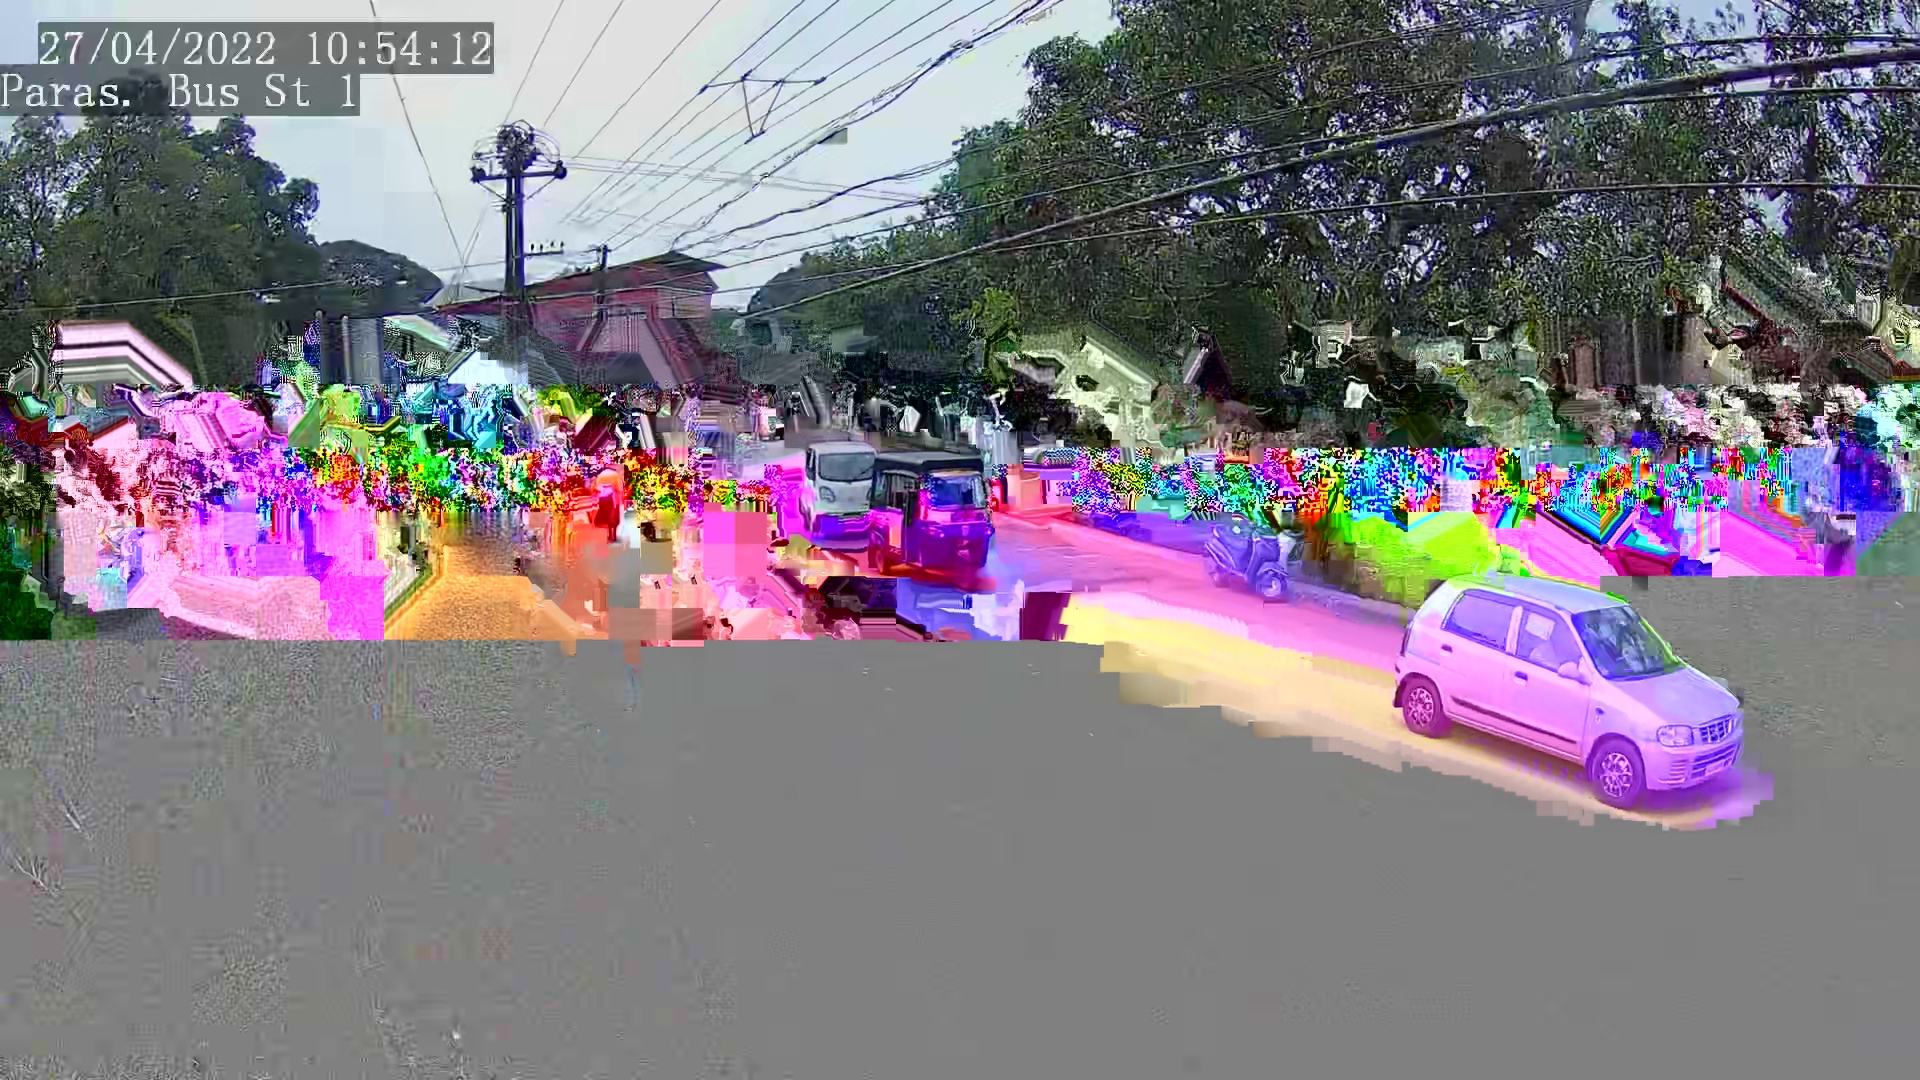
\includegraphics[width=0.32\linewidth]{Images/camera_footage/corrupted1} \hfill
	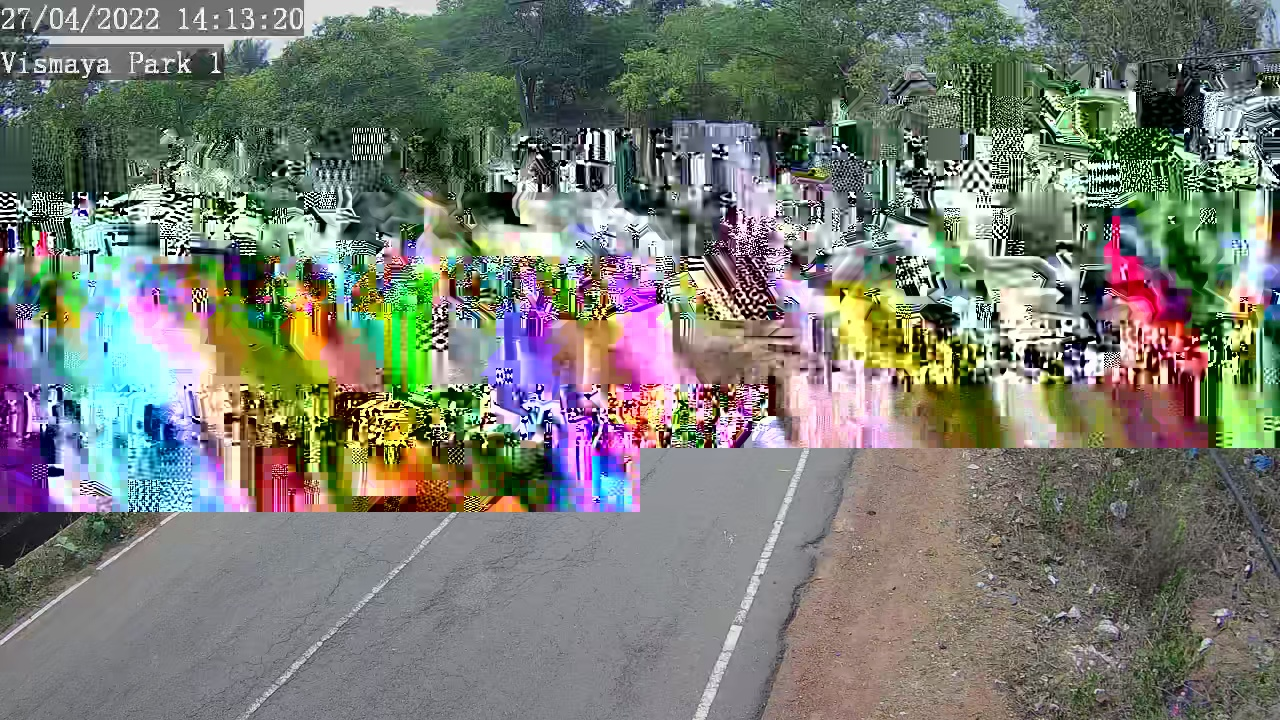
\includegraphics[width=0.32\linewidth]{Images/camera_footage/corrupted2} \hfill
	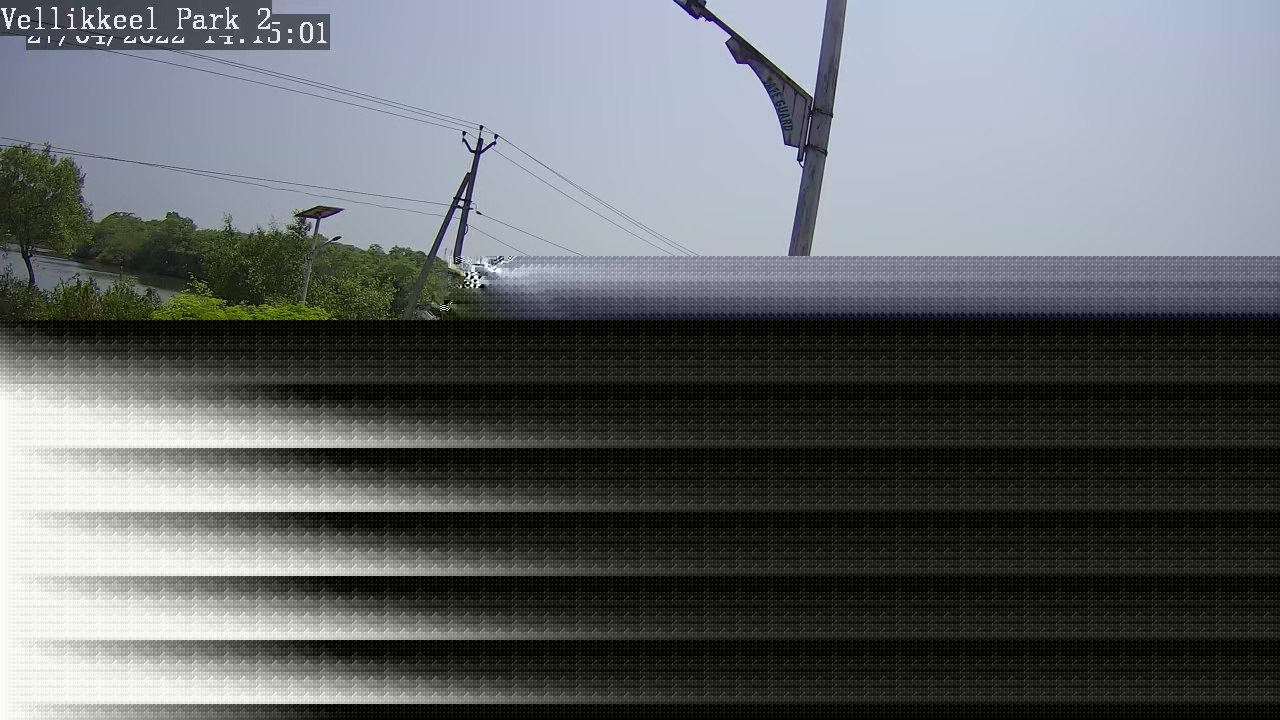
\includegraphics[width=0.32\linewidth]{Images/camera_footage/corrupted3} \\ 
	\\
	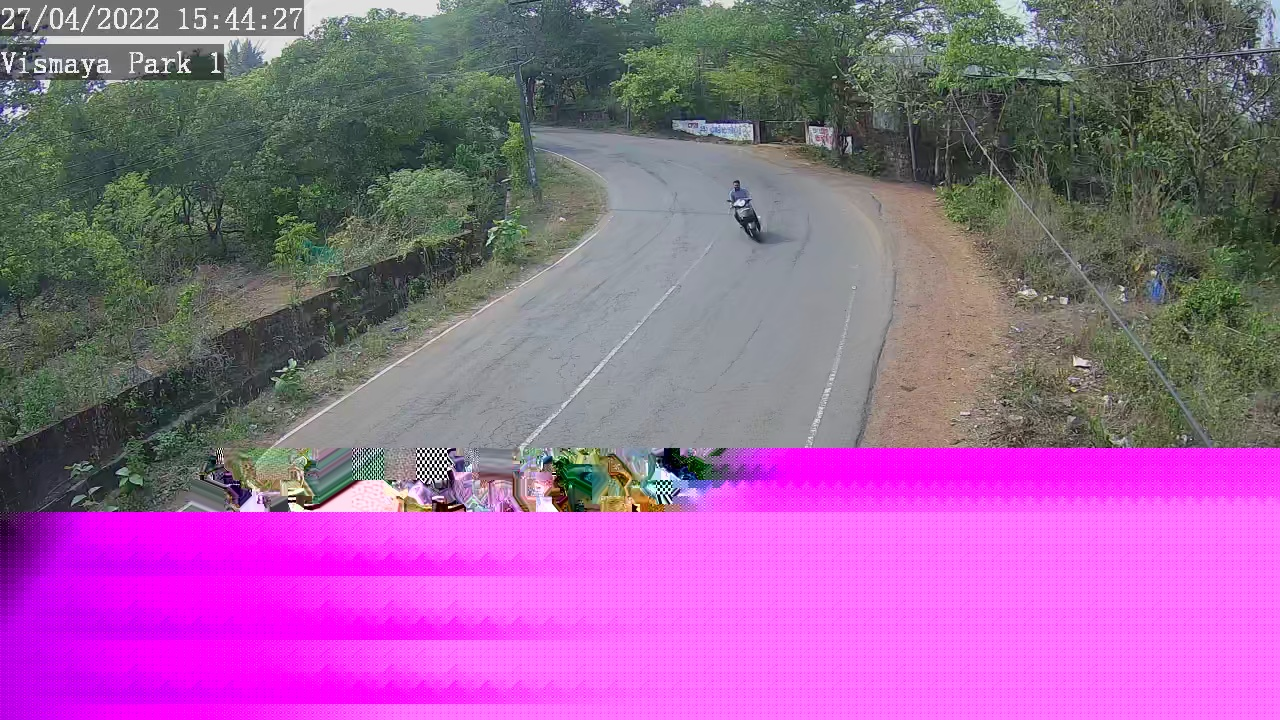
\includegraphics[width=0.32\linewidth]{Images/camera_footage/corrupted4} \hfill
	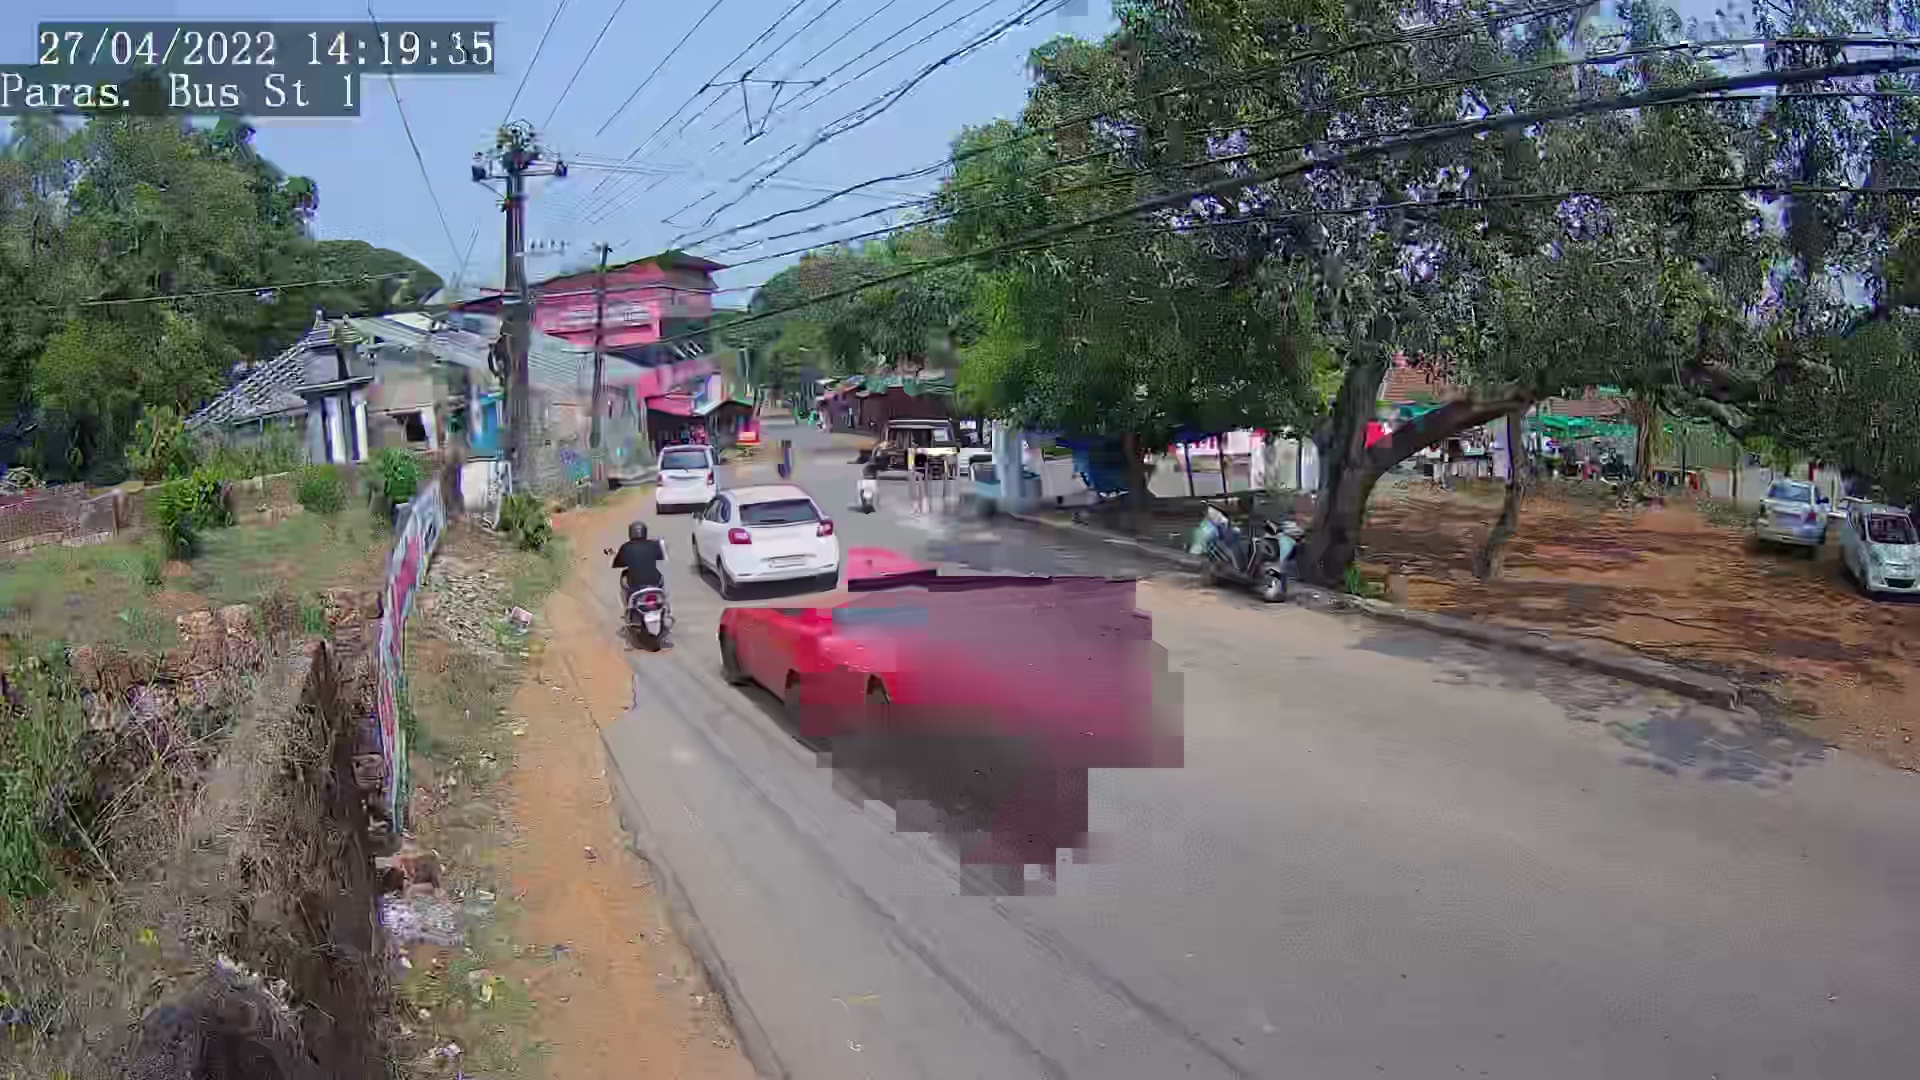
\includegraphics[width=0.32\linewidth]{Images/camera_footage/corrupted5} \hfill
	
\includegraphics[width=0.32\linewidth]{Images/camera_footage/corrupted6} 
	\caption{Corrupted Camera footage}
	\label{fig:corrupted}
\end{figure}

\section{YOLOv4}
YOLOv4 model is trained with 1559 images for 9 classes as illustrated in table \ref{tab:dataset_sum1}. Model accuracy is easily calculated by Darknet and is shown in table \ref{tab:yolo_matrix} and \ref{tag:yolo_score}. The model, in the deployment ran at slower speed of about 19.1 FPS. The decrease in speed is due to the unwanted processing of dead/corrupted frame. Speed can also be improved by reducing the yolo network size, compromising accuracy.

\begin{table}[!ht]
	\centering
	\begin{tabular}{|l|l|l|l|}
		\hline
		Class label    & True Positive & False Positive & Avg Precision \\ \hline
		auto           & 424           & 38             & 98.25\%       \\ \hline
		bus            & 327           & 42             & 99.57\%       \\ \hline
		tempo traveler & 76            & 7              & 97.12\%       \\ \hline
		tractor        & 130           & 2              & 98.44\%       \\ \hline
		truck          & 516           & 33             & 99.28\%       \\ \hline
		van            & 227           & 22             & 98.14\%       \\ \hline
		two wheeler    & 770           & 241            & 91.62\%       \\ \hline
		car            & 644           & 91             & 96.99\%       \\ \hline
		jcb            & 0             & 0              & 100.00\%      \\ \hline
	\end{tabular}
	\caption{YOLOv4 accuracy matrix}
	\label{tab:yolo_matrix}
\end{table}

\begin{table}[!ht]
	\centering
	\begin{tabular}{|l|l|}
		\hline
		Precision            & 87\%    \\ \hline
		Recall               & 96\%    \\ \hline
		F1-score             & 91\%    \\ \hline
		True Positive        & 3114    \\ \hline
		False Positive       & 476     \\ \hline
		False Negative       & 134     \\ \hline
		Avg IoU              & 72.13\% \\ \hline
		Mean Avg precision   & 97.71\% \\ \hline
		Total Detection Time & 1166 Seconds \\ \hline
		Detection count      & 12349 \\ \hline
		Unique truth count   & 3257 \\ \hline
	\end{tabular}
	\caption{YOLOv4 evaluation}
	\label{tag:yolo_score}
\end{table}

\begin{figure}[ht!]
	\centering
	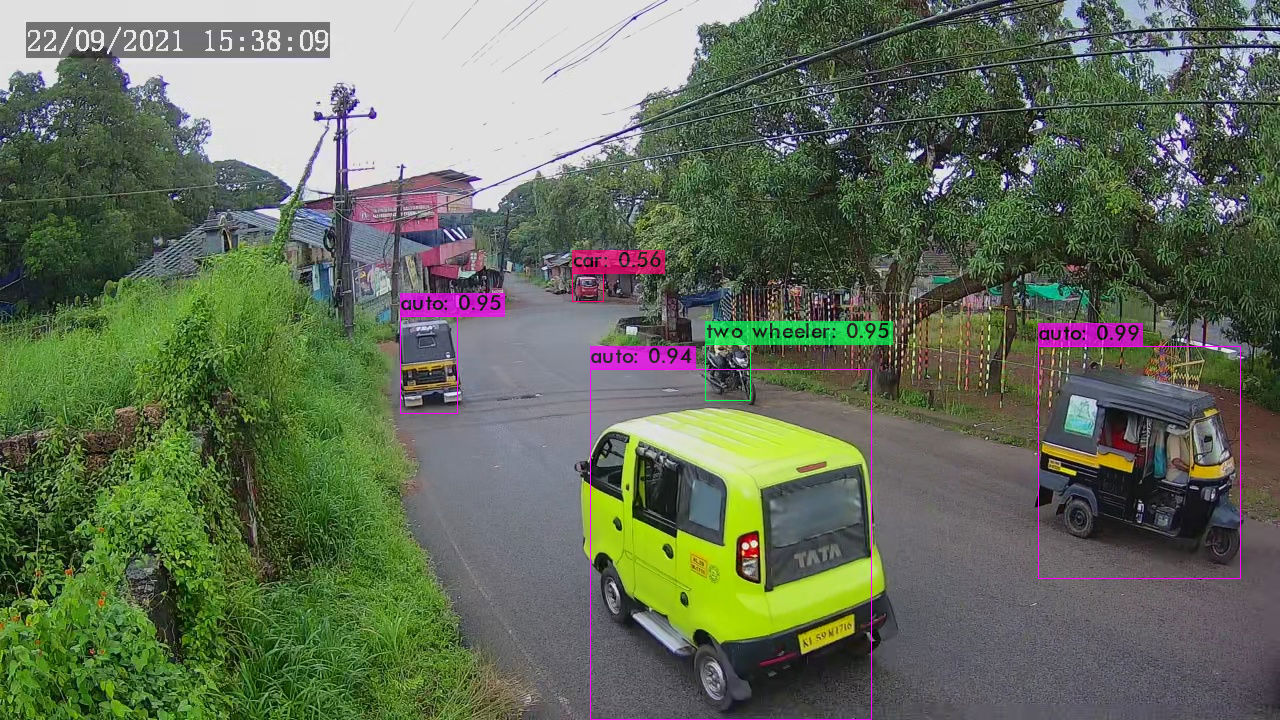
\includegraphics[width=0.8\linewidth]{Images/predictions}
	\caption{YOLOv4 vehicle predictions}
\end{figure}



\section{DeepSORT}
Ground Truth dataset was not available to quantize the result. However, via visual inception, it was found that the model was able to assign correct ID number to most of the vehicles. It was observed that such an increase in accuracy was observed due to the presence of Kalman filtering algorithm. The deep matrix association for humans was trigger only at the presence of humans. It lead to a mismatch where traditional Kalman filter tries to re-Id the bounding boxes, where as deepSORT tries to match human description leading to wrong answer. The anomaly can be strongly seen in public transport bus. Building of deep matrix for vehicle can improve the system.

\section{Siamese Network}
Proper Siamese Network was unable to construct, as the layers of yolov4 models was not able to selectively extract. The YOLOV4 model have tight coupling between layers, with multiple output and input vectors. The model is originally implement in Darknet.  This provided hindrance during the extraction of layers using keras and python. Ground Truth dataset is not able to quantize its accuracy




\chapter{Conclusions and Future Scope}

\section{Conclusion}
The project is developed using the existing technology and methods. This project extends the functionality of camera network offered by CICET. The footage are captured and processed by AI services. YOLOv4 model computes the bounding box along with the class confidence. DeepSORT uses the deep matrix to conduct multi-tracking in multiple objects. Upon the user query, the most relevant detections are provides, which the user can visually verify. This leads to the development of route parsed by the target vehicle. This project thus helps fast tracking of vehicles. The project can be considered as one of candidates for Open AI challenge proposed by NVIDIA. 

\section{Future Scope}
Various levels of improvement can be done, specially in AI domain. Since False Positive do not have heavy impact on the problem domain, a fair trade-off can be applied between the speed and accuracy of the model. Heuristics can be applied after conducting the deeper analysis of the traffic pattern. Various development of PP-YOLO, a PyTorch implementation of YOLO model, is gaining popularity. A new framework called PaddlePaddle \cite{paddlepaddle} is being developed aiming distributed processing, which can significantly increase the processing speed. Various methods are being proposed in PaddlePaddle that significantly reduces the complexity of several algorithms, making real-time application more realizable. Below are some of the pointer that can further enhance the functionality of the project:
\begin{itemize}
	\item Usage of higher resolution camera can better extract the unique feature of vehicles. Cameras can be placed under a bright light source enabling better detection at night.
	\item Integration of license plate detection and Motor Vehicle Department can be used to reverse map the vehicle description, in search of forged vehicle registration.
	\item Train the model in varying weather condition such as sunny, cloudy, rainy etc. Target classes can be increased to detect sub-category of vehicles.
	\item Tighter integration of YOLO model and DeepSORT can reduce redundant extraction and processing of feature vectors.
	\item Current route generation requires visual inspection, which can be replaced by successful implementation of Siamese Network.
	\item Mapping between camera needs to be improved for better route estimation.
	\item Use of PP-YOLO with PaddlePaddle framework can boost the overall performance of the distributed system.
\end{itemize}


%%%%%%%%%%%%%%%%%%%%%%%%%%%%%%%%%%%%%%%%%%%%%%%%%%%%%%%%%%%
%% Bibliography 
%%%%%%%%%%%%%%%%%%%%%%%%%%%%%%%%%%%%%%%%%%%%%%%%%%%%%%%%%%%
\clearpage
%\addcontentsline{toc}{chapter}{Bibliography}
%\bibliographystyle{IEEEtran}
\bibliography{IEEEabrv,reference.bib}
%\printbibliography

%%%%%%%%%%%%%%%%%%%%%%%%%%%%%%%%%%%%%%%%%%%%%%%%%%%%%%%%%%%
\end{document}
